\documentclass[a4j, twocolumn, dvipdfmx]{jsarticle}  % 研究計画は1段組が読みやすい（日本語対応）

\usepackage[a4paper, left=2.0cm, right=2.0cm, top=2.0cm, bottom=2.0cm]{geometry} % 余白を標準寄りに
\usepackage{amsmath}   % 数式用
\usepackage[dvipdfmx]{graphicx}
\usepackage{booktabs}  % \toprule, \midrule, \bottomrule 等の表罫線用
\usepackage{titlesec}  % 見出し調整
\usepackage{enumitem}  % 箇条書きの余白調整（見やすさ改善）
\usepackage{tikz}
\usetikzlibrary{positioning}
\usepackage{algorithm}
\usepackage{algpseudocode}
\usepackage{float}
\usepackage{flushend}  % 最終ページの左右コラムの高さを自動でそろえる（余白の偏り対策）
\raggedbottom  % 大きな図を[H]配置した際に段が伸ばされて生じる不自然な空白を防ぐ

% =========================================================
% 見出し設定
% =========================================================
\titleformat{\section}[block]
  {\normalfont\large\bfseries}
  {\thesection}{0.7em}{}

\titleformat{\subsection}[block]
  {\normalfont\normalsize\bfseries}
  {\thesubsection}{0.7em}{}

\titleformat{\subsubsection}[block]
  {\normalfont\normalsize\bfseries}
  {\thesubsubsection}{0.7em}{}

% 見出し前後の余白
\titlespacing*{\section}
  {0pt}{1.5ex plus 0.5ex minus 0.2ex}{0.8ex}

\titlespacing*{\subsection}
  {0pt}{1.2ex plus 0.4ex minus 0.2ex}{0.6ex}

% =========================================================
% 箇条書き設定
% =========================================================
\setlist[itemize]{
  topsep=3pt,
  itemsep=1pt,
  parsep=0pt,
  leftmargin=*
}


% 箇条書きの詰まりを軽減
\setlist[itemize]{topsep=4pt, itemsep=2pt, leftmargin=*}

\title{
Federated LearningにおけるAdaptive Model Poisoning AttackとRobust Aggregationの評価に関する実験報告書
}
\author{3CDA2216 笠原秀星}
\date{\today}

\begin{document}

\maketitle  % タイトルを表示

\section{研究背景・概要}

Federated Learning（以下, FL）は, 生データを共有することなく複数のデバイスや組織が協調して機械学習モデルを学習する分散学習の枠組みである\cite{mammen2021fl}.
FLは, ユーザのプライバシー保護と機械学習の両立を可能にする技術として注目されており, スマートフォンにおける単語予測や顔認識, 音声認識技術の向上に利用されている. また, 厳格なプライバシー規制によりデータ共有が困難な医療分野や, 自動運転車におけるリアルタイムデータの活用など, 幅広い分野への応用が期待されている\cite{li2019fl}.

一方で, FLには収束性, データ分布の不均一性（Non-I.I.D.）, 通信コスト, 大規模環境への適用, モデル集約手法など, さまざまな課題が存在する\cite{ma2020privacy}. 特に, FLでは多数の参加者が学習に関与するため, 悪意のあるクライアントによる攻撃への耐性を確保することが重要な研究課題となっている. 医療データや個人情報などの機密性の高いデータを扱う応用が想定されることから, 安全かつ信頼性の高い学習環境の実現が求められている.

FLに対する代表的な攻撃としてPoisoning Attackが挙げられる. Poisoning Attackは大きくData Poisoning AttackとModel Poisoning Attackの2種類に分類される. Data Poisoning Attackは学習データそのものを改ざんする攻撃であり, ラベル反転攻撃やBackdoor Attackなどが含まれる. 一方, Model Poisoning Attackはクライアントがサーバへ送信するモデル更新や勾配情報を改ざんする攻撃であり, 勾配操作や最適化手法を利用した攻撃などが提案されている.

これらの攻撃に対する防御手法としては, 異常検知, Robust Aggregation, 摂動機構の3つに大別される. 異常検知にはコサイン類似度やクラスタリング, スコアベース手法などが用いられる. また, Robust AggregationにはKrum, Trimmed Mean, Median, Bulyanなどの集約手法が提案されている. さらに, 摂動機構としては差分プライバシーを利用した手法が広く研究されている\cite{sagar2023survey}.

本研究では, これらの中でもModel Poisoning Attackに着目する. Data Poisoning Attackに関してはこれまで多くの研究が行われており, 攻撃に対してロバストな集約手法や検知手法が多数提案されている. 一方で, Model Poisoning Attackは学習データではなくモデル更新そのものを改ざんするため, サーバ側から攻撃を識別することが困難であり, より深刻な脅威となる. また, その防御手法に関する研究はData Poisoning Attackと比較して十分に進んでいるとは言えない.

さらに, FangらはAdaptive Model Poisoning Attackを提案し, 既存のRobust Aggregation手法を考慮した攻撃によって防御機構を回避できる可能性を示している\cite{fang2020local}. このことは, 従来の防御手法が必ずしも十分な耐性を有していないことを示唆しており, Adaptive Model Poisoning Attackに対する詳細な評価が必要である.

そこで本研究では, IID環境およびNon-IID環境においてAdaptive Model Poisoning AttackがFLの学習性能に与える影響を評価する. また, KrumやTrimmed MeanなどのRobust Aggregation手法に対する攻撃の有効性を比較・分析し, 既存防御手法の限界を明らかにする. さらに, 攻撃が成立する要因について考察するとともに, Model Poisoning Attackに対する効果的な防御手法について検討することを目的とする.

\section{事前知識}
\subsection{Federated Learning}
%FLとは何か.従来の機械学習とは何が違うのか.どういうアルゴリズムを用いるのかなど基礎的なFLの知識について述べる.
%通信ラウンド,クライアント,サーバ
%FLを攻撃と防御の観点からカテゴリー分けする.
先に述べたようにFederated Learningは生データを共有することなく複数のデバイスや組織が協調して機械学習モデルを学習する分散学習の枠組みである\cite{mammen2021fl}.
集約アルゴリズムとしてFederated Averaging (以下,FedAvg)を用いる.FedAvgはGoogleが2016年に発表した論文の中で示されたものである\cite{mcmahan2017fedavg}.

\subsubsection{FedAvg}
\begin{table}[t]
\centering
\caption{FedAvgで用いる主な記号}
\begin{tabular}{ll}
\hline
記号 & 意味 \\
\hline
$K$ & 全クライアント数 \\
$C$ & 各ラウンドで参加する割合 \\
$S_t$ & ラウンド$t$で選択されたクライアント集合 \\
$w_t$ & グローバルモデル \\
$w_{t+1}^k$ & クライアント$k$が更新したモデル \\
$n_k$ & クライアント$k$のデータ数 \\
$E$ & ローカル学習のエポック数 \\
$B$ & ミニバッチサイズ \\
$\eta$ & 学習率 \\
\hline
\end{tabular}
\label{tab:fedavg_symbol}
\end{table}
\begin{algorithm}[t]
\caption{Federated Averaging (FedAvg)}
\label{alg:fedavg}
\begin{algorithmic}[1]

\State \textbf{Server executes:}
\State Initialize $w_0$

\For{each round $t = 1,2,\ldots$}
    \State $m \leftarrow \max(C \cdot K, 1)$
    \State $S_t \leftarrow$ random set of $m$ clients

    \ForAll{$k \in S_t$ in parallel}
        \State $w_{t+1}^{k} \leftarrow \mathrm{ClientUpdate}(k,w_t)$
    \EndFor

    \State $
    w_{t+1}
    \leftarrow
    \sum_{k \in S_t}
    \frac{n_k}{n_t}
    w_{t+1}^{k}
    $
\EndFor

\Statex
\State \textbf{ClientUpdate}$(k,w)$
\State Split $P_k$ into batches of size $B$

\For{$i=1$ to $E$}
    \For{batch $b \in B$}
        \State $
        w \leftarrow
        w-\eta\nabla\ell(w;b)
        $
    \EndFor
\EndFor

\State \Return $w$ to server

\end{algorithmic}
\end{algorithm}
アルゴリズム\ref{alg:fedavg}にFedAvgの処理手順を示す。

まず，サーバはグローバルモデル $w_0$ を初期化する。
その後，各通信ラウンド $t$ において，全クライアント数 $K$ のうち割合 $C$ に応じた $m$ 個のクライアントをランダムに選択する。
選択されたクライアント集合を $S_t$ とする。

選択された各クライアントは，サーバから受け取ったグローバルモデル $w_t$ を用いてローカル学習を実施する。
各クライアントは自身が保有するデータ集合 $P_k$ をミニバッチサイズ $B$ ごとに分割し，エポック数 $E$ 回の学習を行う。
モデル更新には確率的勾配降下法（SGD）を用い，学習率を $\eta$ とすると，各ミニバッチ $b$ に対して次式によりパラメータを更新する。

\begin{equation}
w \leftarrow w-\eta\nabla \ell(w;b)
\end{equation}

ここで，$\ell(w;b)$ はミニバッチ $b$ に対する損失関数であり，$\nabla \ell(w;b)$ はその勾配を表す。

ローカル学習終了後，各クライアントは更新後のモデル $w_{t+1}^{k}$ をサーバへ送信する。
サーバは受信したモデルを，各クライアントの保有データ数 $n_k$ に応じて重み付け平均することで新たなグローバルモデル $w_{t+1}$ を生成する。

\begin{equation}
w_{t+1}
=
\sum_{k \in S_t}
\frac{n_k}{n_t}
w_{t+1}^{k}
\end{equation}

ただし，

\begin{equation}
n_t=\sum_{k\in S_t}n_k
\end{equation}

である。
この処理を複数ラウンド繰り返すことで，生データを共有することなくグローバルモデルを学習する。
\subsection{Data Poisoning Attack}

Data Poisoning Attackは，攻撃者が学習データそのものを改ざんし，グローバルモデルの性能低下や誤動作を引き起こす攻撃である。Federated Learningでは，各クライアントが保有するローカルデータや学習過程をサーバが直接確認できないため，悪意のあるクライアントが改ざんしたデータを用いて学習を行うことで，モデルに悪影響を与えることが可能である\cite{sagar2023survey}。

Data Poisoning Attackは，Label Flipping Attack，Poisoning Sample Attack，Backdoor Attackなどに分類される。Label Flipping Attackは，学習データのラベルを意図的に別のラベルへ変更する攻撃である。例えば，数字認識タスクにおいて「1」のラベルを「7」に変更して学習させることで，モデルの分類性能を低下させることができる。

Poisoning Sample Attackは，学習データそのものを改ざんする攻撃であり，ノイズの付加や特定のパターンの埋め込みなどによって学習結果を操作する。

一方，Backdoor Attackは，特定のトリガを含む入力に対してのみ誤分類を引き起こす攻撃である。攻撃者はトリガ付きデータを学習データへ混入させることで，通常の入力に対する性能を維持したまま，トリガを含む入力に対してのみ攻撃者が指定したラベルを出力するようモデルを誘導する。そのため，Backdoor Attackは高い攻撃成功率とステルス性を有しており，発見が困難であるという特徴を持つ。

Data Poisoning Attackは実装が比較的容易である一方，異常なデータ分布やラベルの偏りを利用した検知手法によって防御できる場合がある。そのため近年では，学習データではなくモデル更新そのものを改ざんするModel Poisoning Attackに関する研究が盛んに行われている\cite{sagar2023survey}\cite{xie2020dba}\cite{nguyen2022flame}。



\subsection{Model Poisoning Attack}

Model Poisoning Attackは，悪意のあるクライアントがサーバへ送信するモデル更新や勾配情報を改ざんし，グローバルモデルの性能低下や誤動作を引き起こす攻撃である。Data Poisoning Attackが学習データそのものを改ざんするのに対し，Model Poisoning Attackは学習後のモデルパラメータを直接操作する点に特徴がある。そのため，サーバ側から攻撃の有無を判断することが困難であり，Federated Learningにおける深刻な脅威の一つとして注目されている\cite{sagar2023survey}。

Model Poisoning Attackは，Gradient Manipulation，Optimization Methods，Untargeted Attackの3種類に分類される\cite{sagar2023survey}。Gradient Manipulationは，モデル更新の勾配を意図的に操作する攻撃であり，勾配反転（Sign Flipping Attack）やランダムな勾配の挿入などが代表例として知られている。これらの攻撃は，グローバルモデルの収束を妨害し，性能を低下させることを目的とする。

Optimization Methodsは，攻撃効果を最大化するようにモデル更新を最適化する攻撃である。攻撃者は正常なモデル更新との差を小さく保ちながら，攻撃目的を達成するようにモデルを改ざんすることで，異常検知や防御機構による検出を回避する。Backdoor AttackやModel Replacement Attackの多くはこの分類に含まれる。

Untargeted Attackは，特定の入力に対する誤分類ではなく，グローバルモデル全体の性能低下を目的とする攻撃である。攻撃者はモデル更新を大きく改ざんすることで，学習の収束を妨害し，モデルの可用性を低下させる。


\subsection{Robust Aggregation}
%Robust Aggregationとは何で,どんな種類があるのか述べる.数式などもあれば良い.
%Krum,Mean,Trimmed Mean,Median,Bulyanなどについて論文で述べられていたはず.
%それぞれの手法については\subsubsectionで書けばいいと思う.
Robust Aggregationは，悪意のあるクライアントによる異常なモデル更新の影響を軽減することを目的とした集約手法である\cite{sagar2023survey}。従来のFedAvgでは，各クライアントから送信されたモデル更新を重み付き平均によって集約するため，悪意のあるクライアントが極端なモデル更新を送信した場合，グローバルモデルが大きな影響を受ける可能性がある。

この問題に対処するため，Byzantine Fault Toleranceの考え方を取り入れたRobust Aggregationが提案されている。代表的な手法としてMean（FedAvg），Median，Trimmed Mean，Krum，Bulyanなどが知られており，異常なモデル更新を除外または影響を低減しながらグローバルモデルを更新する。

\subsubsection{Mean (FedAvg)}

FedAvgは，Federated Learningにおいて最も広く利用されている集約手法である。各クライアントから送信されたモデル更新を，保有するデータ数に応じて重み付け平均することで新たなグローバルモデルを生成する。

FedAvgは実装が容易で計算コストも低いという利点を持つ一方，異常なモデル更新の影響を受けやすいという欠点がある。そのため，Model Poisoning Attackに対して脆弱であることが知られている。

\subsubsection{Median}

Medianは，各パラメータについて中央値を採用する集約手法である。平均値ではなく中央値を利用することで，極端に大きな値や小さな値の影響を受けにくくなる。

そのため，悪意のあるクライアントが異常なモデル更新を送信した場合でも，その影響を軽減できる。しかし，多数のクライアントが攻撃に参加している場合には性能が低下する可能性がある。

\subsubsection{Trimmed Mean}

Trimmed Meanは，各パラメータについて極端に大きい値と小さい値を一定数除外した後に平均を計算する手法である。

この手法は外れ値の影響を低減できるため，単純な平均よりもModel Poisoning Attackに対してロバストである。一方で，正常なクライアントの更新が除外される場合もあり，学習性能が低下する可能性がある。

\subsubsection{Krum}

Krumは，各クライアントのモデル更新と他のクライアントとの距離を計算し，最も多くのクライアントと類似しているモデル更新を選択する手法である。

平均を取るのではなく，信頼できると判断された単一のモデル更新を採用するため，異常なモデル更新を排除しやすいという特徴を持つ。しかし，クライアント数が増加すると計算コストが大きくなるという課題がある。

\subsubsection{Bulyan}

Bulyanは，KrumとTrimmed Meanを組み合わせた集約手法である。まずKrumを用いて信頼できるモデル更新を選択し，その後Trimmed Meanによって集約を行う。

複数のByzantine攻撃に対して高い耐性を持つことが報告されているが，計算コストが大きく，クライアント数が多い環境では実行時間が増加するという欠点がある。

本研究では，FedAvgを基準手法とし，Median，Trimmed Mean，KrumおよびBulyanをRobust Aggregationとして採用する。また，Adaptive Model Poisoning Attackを適用した場合の攻撃成功率やモデル精度の変化を比較し，各集約手法の有効性を評価する。


%あとでそれぞれの手法の代表論文についても確認して示さなきゃいけないと思うけど,とりあえずはこれで.
%まだ論文を読んでないので必要に応じて収集する.
\section{関連研究}

Subhash Sagarらは，Federated LearningにおけるPoisoning Attackおよび防御手法に関する包括的なサーベイを行っている。彼らは攻撃をData Poisoning AttackとModel Poisoning Attackに分類し，さらに防御手法についてもRobust Aggregationや異常検知手法などの観点から体系的に整理している。また，各攻撃手法および防御手法の特徴や課題を比較し，Federated Learningにおけるセキュリティ研究の方向性を示している\cite{sagar2023survey}.

Minghong Fangらは，Byzantine-robust Federated Learningに対するLocal Model Poisoning Attackを提案した。従来のData Poisoning Attackとは異なり，攻撃者は学習データではなく悪意あるクライアントのモデル更新そのものを操作する。攻撃を最適化問題として定式化することで，Krum，Bulyan，Median，Trimmed MeanといったByzantine-robust Aggregation手法に対しても有効な攻撃を実現し，既存の防御手法が十分ではないことを示した\cite{fang2020local}.

Chulin Xieらは，DBA (Distributed Backdoor Attacks) を提案した。従来のBackdoor Attackでは全ての攻撃者が同一のトリガを学習するのに対し，DBAではグローバルトリガを複数のローカルトリガへ分割し，各悪意あるクライアントへ分散して埋め込む。この手法により，従来手法と比較して高い攻撃成功率とステルス性を実現できることを示した\cite{xie2020dba}.

Eugene Bagdasaryanらは，Model Replacement Attackを提案した。この攻撃では，攻撃者が生成した悪意あるモデル更新を拡大して送信することで，集約後のグローバルモデルへBackdoorを埋め込むことが可能となる。また，Federated Learningで用いられるSecure Aggregation環境では各クライアントの更新内容を詳細に観測できないため，異常検知による防御が困難であることを示した\cite{bagdasaryan2020model}.

Tuan D. Nguyenらは，Backdoor Attackに対する防御手法であるFLAMEを提案した。FLAMEはモデルクラスタリングによる異常なモデル更新の検出，重みクリッピングによる影響の抑制，およびノイズ付与を組み合わせることで，正常なモデル性能を維持しながらBackdoorの影響を低減できることを示した\cite{nguyen2022flame}.

これらの研究では，Poisoning AttackおよびBackdoor Attackの有効性や防御手法について検討されている。しかし，Adaptive Model Poisoning Attackに対する各種Robust Aggregation手法の耐性については十分な比較評価が行われていない。そこで本研究では，Median，Trimmed Mean，Krum，BulyanなどのRobust Aggregation手法を対象としてAdaptive Model Poisoning Attackを適用し，IID環境およびNon-IID環境における防御性能を評価する。




\section{実験方法}

\subsection{実験概要}

本研究では，Federated Learning環境においてAdaptive Model Poisoning Attackを実施し，各種Robust Aggregation手法の耐性を評価する．

実験では，全100クライアントから構成されるFederated Learning環境を構築し，悪性クライアント割合およびデータ分布を変化させながら学習を行う．

また，FedAvg，Median，Trimmed Mean，Krum，Bulyanの
5種類の集約手法を対象とし，攻撃下におけるモデル性能の変化を比較する．

\subsection{データセット}

本研究では，画像分類タスクの代表的なデータセットであるMNISTを用いる．MNISTは手書き数字画像から構成される10クラス分類データセットであり，訓練データ60,000件，テストデータ10,000件を含む．

データ分布が攻撃および防御性能に与える影響を評価するため，IID環境およびNon-IID環境の両方で実験を行う．IID環境では各クライアントへデータを均等に分配する．一方，Non-IID環境ではクライアントごとに保有ラベルを偏らせることで，不均一なデータ分布を再現する．

\subsection{学習モデル}

学習モデルには，全結合型Deep Neural Network（DNN）を用いる．モデル構造は，入力層，128ノードの全結合層，64ノードの全結合層，および10クラス分類のための出力層から構成される．活性化関数にはReLUを用いる．

本モデルは，ロジスティック回帰より高い表現能力を有しながら，CNNやResNetと比較して実装および実験管理が容易であるため採用する．

\subsection{攻撃設定}

攻撃手法には，Fangらが提案したAdaptive Model Poisoning Attackを用いる．

Adaptive Model Poisoning Attackは，従来のModel Poisoning Attackとは異なり，サーバで用いられる集約手法の特性を考慮して悪意あるモデル更新を生成する攻撃である．攻撃者は，グローバルモデルの性能低下を目的としてモデル更新を最適化し，Robust Aggregationによる防御を回避しながら攻撃を行う．

\subsubsection*{正常クライアントと悪性クライアントの定義・選出方法}

本研究では，各ラウンドの通信に参加するクライアントを，攻撃に関与しない\textbf{正常（honest）クライアント}と，Adaptive Model Poisoning Attackによる攻撃済みの更新を送信する\textbf{悪性（malicious）クライアント}の2種類に分類する．正常クライアントはローカル学習の結果をそのままサーバへ送信するのに対し，悪性クライアントはローカル学習自体は正常クライアントと同様に行うものの，サーバ側で更新が集約される直前に，その更新が攻撃によってクラフトされた値へ差し替えられる．

悪性クライアントの選出は，クライアント総数と悪性クライアント割合から悪性クライアント数を算出した上で，シード値を用いた乱数生成によりクライアントIDの中から重複なく抽出することで行う．クライアント総数・悪性クライアント割合・シード値の組み合わせが同一であれば常に同一の悪性クライアント集合が得られるため，実験の再現性が確保される．一方で，シード値を変更すると，モデルの初期値やデータ分割だけでなく，悪性クライアントとして選出されるクライアントID自体も変化する点に注意が必要である．

本研究では，悪性クライアントが正常なローカル学習を実施した後，学習結果をそのまま送信する代わりに，Adaptive Model Poisoning Attackによって生成した悪意あるモデル更新をサーバへ送信する．

\subsubsection*{full knowledge攻撃者の実現方法}

Fangらの攻撃は，攻撃者がサーバで使用中の集約手法を把握しており，かつ悪性クライアント同士が結託して互いの更新内容を参照できる，いわゆるfull knowledge攻撃者を前提とする．本実験基盤であるFlowerでは，各クライアントは独立したプロセスとして動作し，クライアント同士が直接通信・結託する手段を持たない．そのため，本研究ではこの前提をサーバ側で模倣する形で実現する．

具体的には，各クライアントは通常どおりローカル学習を行い，学習結果をサーバへ送信する．サーバは全クライアントの更新を受信し集約する直前に，送信元のクライアントIDから悪性クライアントに該当する更新を特定した上で，それらを正常クライアントの更新情報とグローバルモデルの情報から生成した攻撃済みの更新へ差し替える．全クライアントの更新が集まるサーバのこのタイミングを，攻撃者が他クライアントの更新を参照して結託する場とみなすことで，クライアントプロセスが独立しているという制約の下でもfull knowledge攻撃者を模擬している．

\subsubsection*{集約手法別のクラフト方法}

Adaptive Model Poisoning Attackでは，攻撃者はまず正常クライアントの更新の平均とグローバルモデルとの差からグローバルモデルを押しやる方向（攻撃方向）を求める．その上で，サーバが使用する集約手法に応じて，以下のように悪性クライアントの更新をクラフトする．

\begin{itemize}
\item \textbf{Median，Trimmed Mean：} 座標ごとに正常クライアントの更新の最大値・最小値を求め，攻撃方向側の最大値・最小値のさらに外側の値を悪性クライアントへ割り当てる境界値攻撃を行う．悪性クライアント間で外側への押し出し具合を段階的にずらすことで，座標ごとの外れ値除外処理によって悪性の更新がまとめて除外されることを防ぐ．
\item \textbf{Krum，Bulyan：} 悪性クライアント全員を正常クライアントの更新の重心を起点とした攻撃方向上の1点に密集させ，Krumによって悪性クライアントの更新が選択される範囲でグローバルモデルから最大限離れるように，攻撃強度を表すパラメータを探索する．BulyanはKrumによる候補選択を繰り返し用いるため，同様のクラフト方法を適用する．
\item \textbf{FedAvg：} 外れ値を除外する仕組みを持たないため，選択回避のための探索は不要であり，悪性クライアントの更新をグローバルモデルとの差分に対して一定倍率で拡大するScale Attackを適用する．
\end{itemize}

なお，本実装はFangらが示した「集約手法の特性を突いた最適化ベースの攻撃」という中核的な着想を踏襲した独自実装であり，原論文の数式をそのまま再現したものではなく，近似・簡略化した再実装である点に留意されたい．

また，攻撃の影響を評価するため，全100クライアント中の悪性クライアント数を0，10，20，30と変化させる．これに対応する悪性クライアント割合はそれぞれ0\%，10\%，20\%，30\%である．

さらに，IID環境およびNon-IID環境の両方において実験を実施し，データ分布の違いが攻撃効果に与える影響についても評価する．

\subsection{防御設定}

防御手法として，Robust Aggregationに分類されるFedAvg，Median，Trimmed Mean，Krum，Bulyanを用いる．

FedAvgは全クライアントのモデル更新の平均を用いる集約手法である．Medianは各パラメータについて中央値を採用する．Trimmed Meanは極端な値を除外した後に平均を計算する．Krumは他のクライアントとの距離に基づいて信頼できるモデル更新を選択する手法である．
BulyanはKrumによる候補選択とTrimmed Meanによる集約を組み合わせた手法であり，高いByzantine耐性を有することが報告されている．
これら5手法を比較することで，
Adaptive Model Poisoning Attackに対する耐性の違いを評価する．

\section{評価方法}

\subsection{評価指標}

評価指標にはAccuracyおよびLossを用いる．

Accuracyはテストデータに対する分類精度を表す指標であり，学習されたグローバルモデルの性能を評価するために用いる．

Lossは損失関数の値を表す指標であり，学習の収束状況を評価するために用いる．Lossが小さいほどモデルの予測結果と正解ラベルとの差が小さく，学習が適切に進行していることを示す．

実験では，各通信ラウンドにおけるAccuracyおよびLossの推移を記録する．Adaptive Model Poisoning AttackによってAccuracyが低下し，Lossが増加するほど，攻撃の影響が大きいと判断する．



\subsection{比較条件}

本研究では，

\begin{itemize}
\item 集約手法（FedAvg，Median，Trimmed Mean，Krum，Bulyan）
\item 悪性クライアント割合（0\%，10\%，20\%，30\%）
\item データ分布（IID，Non-IID）
\end{itemize}

を組み合わせて比較を行う．

実験条件数は

\[
5 \times 4 \times 2 = 40
\]

条件である。

各条件について3回ずつ実験を行うため，

\[
40 \times 3 = 120
\]

回の実験を実施する。

\section{実験環境}

実験はPythonを用いて実装する．深層学習フレームワークにはPyTorchを使用し，Federated Learningの実装にはFlowerを用いる．

全クライアント数は100とし，各通信ラウンドでは全クライアントが学習へ参加する．

通信ラウンド数，ローカルエポック数，バッチサイズ，学習率などのハイパーパラメータは，予備実験により以下のように決定した．

\begin{itemize}
    \item \textbf{通信ラウンド数：} 20
    \item \textbf{ローカルエポック数：} 1
    \item \textbf{バッチサイズ：} 25
    \item \textbf{学習率：} 0.001
    \item \textbf{最適化手法：} AdamW
\end{itemize}


\section{実験}
\subsection{FedAvg(IID-環境)における悪性クライアントの比率別評価}
\subsubsection{実験条件}

FedAvgを用いたIID環境において，悪性クライアント比率を変化させ，
悪性クライアント比率がモデルの性能に与える影響を比較する．
以下の条件はすべての実験で共通とした．

\begin{itemize}
    \item \textbf{Aggregation Method：} FedAvg
    \item \textbf{Data Split：} IID
    \item \textbf{Attack：} Adaptive Attack
    \item \textbf{Number of Rounds：} 20
    \item \textbf{Seeds：} 1，2，3
\end{itemize}

比較対象とする悪性クライアント比率を以下に示す．

\begin{itemize}
    \item \textbf{Malicious Ratio：} 0.0，0.1，0.2，0.3
\end{itemize}

乱数の影響を考慮し，Seed値を1，2，3の3通り設定して実験を行った．
本文中の図には代表としてSeed 1の結果を示す．Seed間の傾向の違いは
次項で述べる．詳細な結果（全Seedの推移）は付録に記載する．
\subsubsection{実験結果}
\begin{figure}[t]
    \centering
    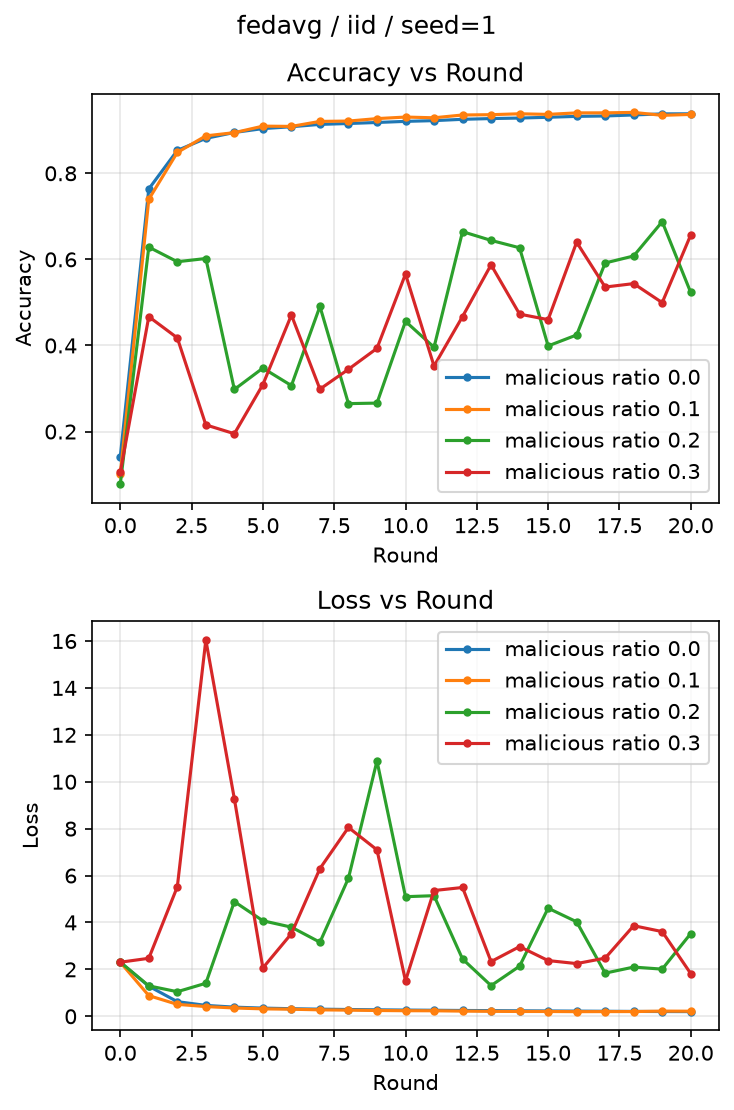
\includegraphics[width=0.85\columnwidth]{result/fedavg_iid_seed1_by_ratio.png}
    \caption{FedAvg・IID・Seed 1 における malicious ratio 別の Round-Accuracy および Round-Loss の推移}
    \label{fig:fedavg_iid_seed1_by_ratio}
\end{figure}

実験結果を図\ref{fig:fedavg_iid_seed1_by_ratio}に示す．また，図の作成に用いたRound別のAccuracyおよびLossの数値を付録の表\ref{tab:fedavg_iid_seed1_by_ratio}に示す．
悪性クライアント(malicious ratio)の割合が0.0,0.1の時は,AccuracyがRound 5までに0.9前後へ収束できていることがわかる.
また,Lossもおおよそ0付近で収束していることから,問題なく学習が行われたことがわかる.
一方,悪性クライアントの割合が0.2の時,全体的にAccuracyは増加傾向が見られ,Lossは減少傾向があることから,学習自体は機能していることが読み取れる.
しかし,悪性クライアントの割合が0.0,0.1の時に比べ,最終的なAccuracyが約30\%ほど下回っていることがわかる.
さらに,悪性クライアントの割合が0.3のときは,round20回では収束の傾向は見られず,学習をしているとは判断できない.
つまり,全体の3割が悪性クライアントの場合は学習は崩壊するということが読み取れる.

\subsection{FedAvg(Non-IID環境)における悪性クライアント比率別評価}
\subsubsection{実験条件}

FedAvgを用いたNon-IID環境において，悪性クライアント比率を変化させ，
悪性クライアント比率がモデルの性能に与える影響を比較する．
以下の条件はすべての実験で共通とした．

\begin{itemize}
    \item \textbf{Aggregation Method：} FedAvg
    \item \textbf{Data Split：} Non-IID
    \item \textbf{Attack：} Adaptive Attack
    \item \textbf{Number of Rounds：} 20
    \item \textbf{Seeds：} 1，2，3
\end{itemize}

比較対象とする悪性クライアント比率を以下に示す．

\begin{itemize}
    \item \textbf{Malicious Ratio：} 0.0，0.1，0.2，0.3
\end{itemize}

乱数の影響を考慮し，Seed値を1，2，3の3通り設定して実験を行った．
本文中の図には代表としてSeed 1の結果を示す．詳細な結果（全Seedの
推移）は付録に記載する．
\subsubsection{実験結果}
\begin{figure}[t]
    \centering
    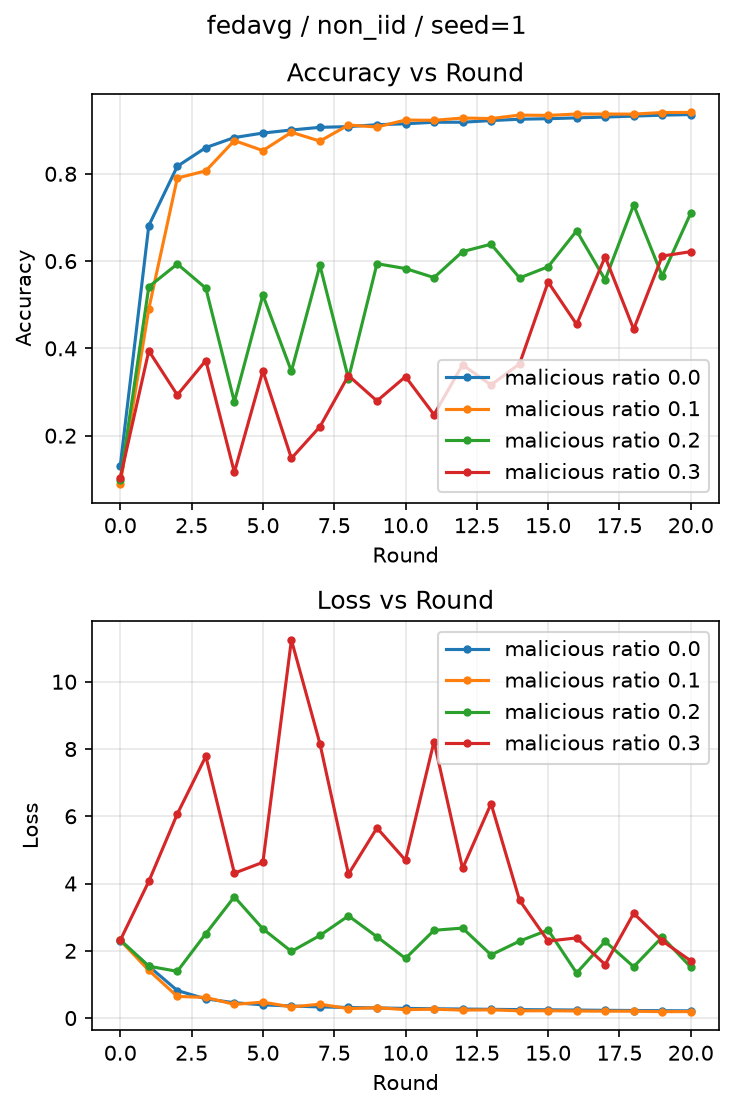
\includegraphics[width=0.85\columnwidth]{result/fedavg_noniid_seed1_by_ratio.png}
    \caption{FedAvg・Non-IID・Seed 1 における malicious ratio 別の Round-Accuracy および Round-Loss の推移}
    \label{fig:fedavg_noniid_seed1_by_ratio}
\end{figure}

実験結果を図\ref{fig:fedavg_noniid_seed1_by_ratio}に示す．また，図の作成に用いたRound別のAccuracyおよびLossの数値を付録の表\ref{tab:fedavg_noniid_seed1_by_ratio}に示す．
悪性クライアントの割合が0.2,0.3の時の最終Accuracyないし
途中経過の推移の幅に関しては，3つのseed値のみでは分布と学習の関連性について結論が出せず，
改善・悪化の原因が分布の違いであるとは判断できないため，追加で検証をする必要がある.

\subsection{Median(IID環境)における悪性クライアント比率別の評価}
\subsubsection{実験条件}

Medianを用いたIID環境において，悪性クライアント比率を変化させ，
悪性クライアント比率がモデルの性能に与える影響を比較する．
以下の条件はすべての実験で共通とした．

\begin{itemize}
    \item \textbf{Aggregation Method：} Median
    \item \textbf{Data Split：} IID
    \item \textbf{Attack：} Adaptive Attack
    \item \textbf{Number of Rounds：} 20
    \item \textbf{Seeds：} 1，2，3
\end{itemize}

比較対象とする悪性クライアント比率を以下に示す．

\begin{itemize}
    \item \textbf{Malicious Ratio：} 0.0，0.1，0.2，0.3
\end{itemize}

乱数の影響を考慮し，Seed値を1，2，3の3通り設定して実験を行った．
本文中の図には代表としてSeed 1の結果を示す．詳細な結果（全Seedの推移）は付録に記載する．

\subsubsection{実験結果}

実験結果を図\ref{fig:median_iid_seed1_by_ratio}に示す．また，図の作成に用いたRound別のAccuracyおよびLossの数値を付録の表\ref{tab:median_iid_seed1_by_ratio}に示す．

\begin{figure}[t]
    \centering
    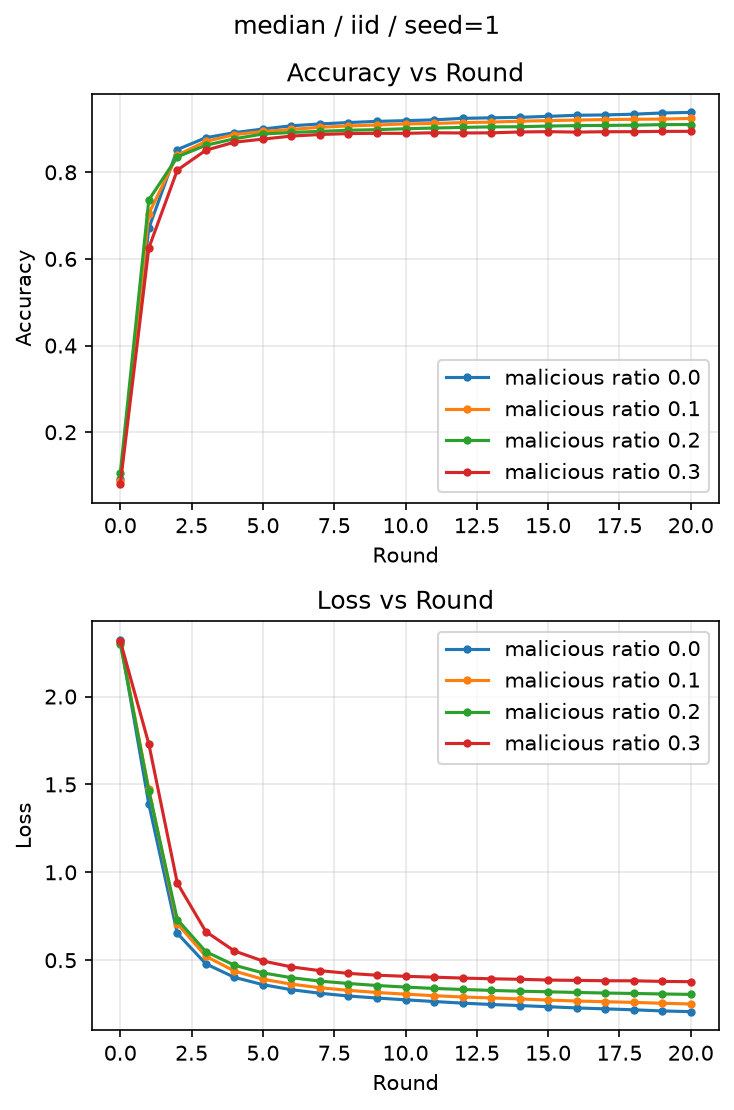
\includegraphics[width=0.85\columnwidth]{result/median_iid_seed1_by_ratio.png}
    \caption{Median・IID・Seed 1 における malicious ratio 別の Round-Accuracy および Round-Loss の推移}
    \label{fig:median_iid_seed1_by_ratio}
\end{figure}

図\ref{fig:median_iid_seed1_by_ratio}より全ての悪性クライアントの割合において,Round5までにほぼ収束し,
Losも同様に単調減少し,収束に向かっている.いずれの条件下でも学習ができており,FedAvgで見られたような振動なども観測されない.
個々の悪性クライアントの割合についてみると,割合が上がるにつれて最終Accuracyが低下しているが,その差は0.05以下に収まっていることがわかる.
Seed間のばらつきも全ての割合において標準偏差0.003以下と極めて小さく,MedianがIID環境において検証した範囲内でAdaptive Model Poisoning Attackに対して比較的ロバストであることを示している.

\subsection{Median(Non-IID環境)における悪性クライアント比率別評価}
\subsubsection{実験条件}

Medianを用いたNon-IID環境において，悪性クライアント比率を変化させ，
悪性クライアント比率がモデルの性能に与える影響を比較する．
以下の条件はすべての実験で共通とした．

\begin{itemize}
    \item \textbf{Aggregation Method：} Median
    \item \textbf{Data Split：} Non-IID
    \item \textbf{Attack：} Adaptive Attack
    \item \textbf{Number of Rounds：} 20
    \item \textbf{Seeds：} 1，2，3
\end{itemize}

比較対象とする悪性クライアント比率を以下に示す．

\begin{itemize}
    \item \textbf{Malicious Ratio：} 0.0，0.1，0.2，0.3
\end{itemize}

乱数の影響を考慮し，Seed値を1，2，3の3通り設定して実験を行った．
本文中の図には代表としてSeed 1の結果を示すが，Malicious Ratio 0.3のSeed 1はRound 1でログが途切れているため，図および付録の表では該当系列のみRound 0--1までの記載となる．詳細な結果（全Seedの推移）は付録に記載する．

\subsubsection{実験結果}

実験結果を図\ref{fig:median_noniid_seed1_by_ratio}に示す．また，図の作成に用いたRound別のAccuracyおよびLossの数値を付録の表\ref{tab:median_noniid_seed1_by_ratio}に示す．

\begin{figure}[t]
    \centering
    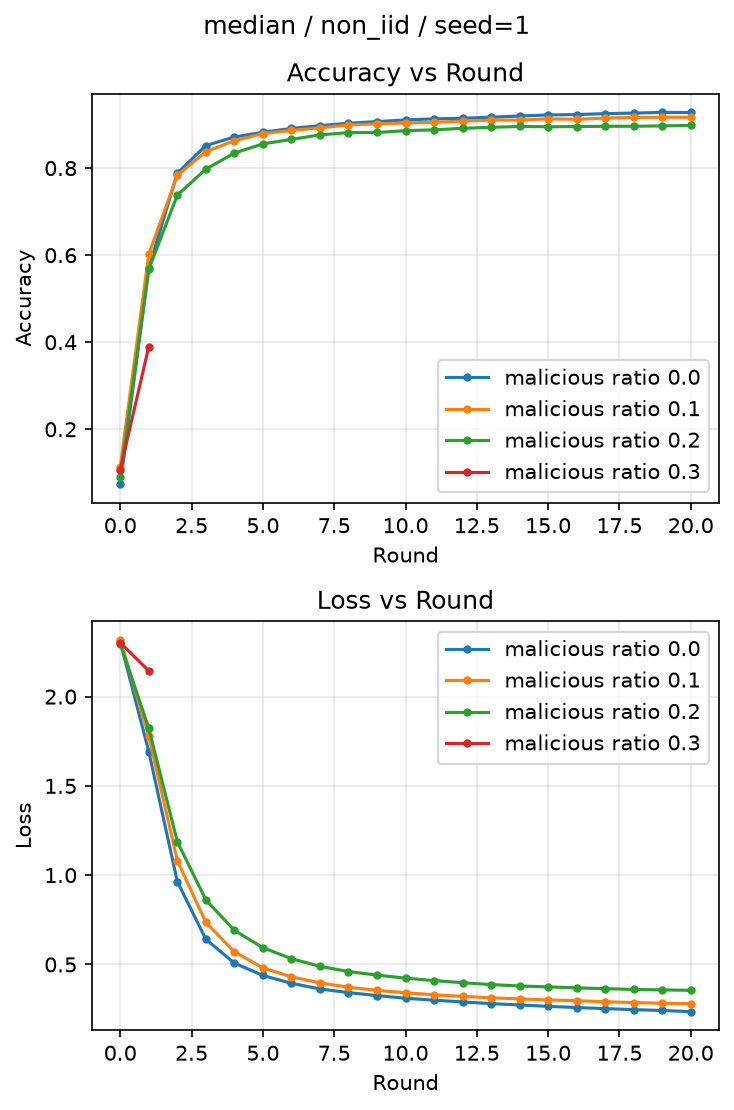
\includegraphics[width=0.85\columnwidth]{result/median_noniid_seed1_by_ratio.png}
    \caption{Median・Non-IID・Seed 1 における malicious ratio 別の Round-Accuracy および Round-Loss の推移（malicious ratio 0.3 は Round 0--1 のみ）}
    \label{fig:median_noniid_seed1_by_ratio}
\end{figure}
図\ref{fig:median_noniid_seed1_by_ratio}より,IID環境同様,0.3を除く全ての悪性クライアントの割合において,Round5までにほぼ収束し,Lossも同様に減少していることから,学習が正しく行われていることがわかった.
Medianは全体としてNon-IID環境においても,検証した範囲内でAdaptive Model Poisoning Attackに対して比較的ロバストであることが示された.\\
(追記)\\
malicious\_rate=0.3のときのseed1のデータが不十分であるため,考察をするために,再度実験を回す必要がある.


\subsection{Trimmed Mean(IID環境)における悪性クライアント比率別評価}
\subsubsection{実験条件}

Trimmed Meanを用いたIID環境において，悪性クライアント比率を変化させ，
悪性クライアント比率がモデルの性能に与える影響を比較する．
以下の条件はすべての実験で共通とした．

\begin{itemize}
    \item \textbf{Aggregation Method：} Trimmed Mean
    \item \textbf{Data Split：} IID
    \item \textbf{Attack：} Adaptive Attack
    \item \textbf{Number of Rounds：} 20
    \item \textbf{Seeds：} 1，2，3
\end{itemize}

比較対象とする悪性クライアント比率を以下に示す．

\begin{itemize}
    \item \textbf{Malicious Ratio：} 0.0，0.1，0.2，0.3
\end{itemize}

乱数の影響を考慮し，Seed値を1，2，3の3通り設定して実験を行った．
本文中の図には代表としてSeed 1の結果を示す．詳細な結果（全Seedの推移）は付録に記載する．

\subsubsection{実験結果}

実験結果を図\ref{fig:trimmed_mean_iid_seed1_by_ratio}に示す．また，図の作成に用いたRound別のAccuracyおよびLossの数値を付録の表\ref{tab:trimmed_mean_iid_seed1_by_ratio}に示す．
MedianのIID環境と同様,全ての悪性クライアントの割合で振動のない滑らかな収束を示す.
Lossも収束の傾向が見られ,正しく学習が進んでいることを意味している.
Accuracyは悪性クライアントの割合が増えるにつれて低下するが,Seed間の標準偏差はいずれも0.004以下と小さい.
Trimmed MeanはIID環境において,検証の範囲内でMedianと同水準のロバスト性を示した.
\begin{figure}[t]
    \centering
    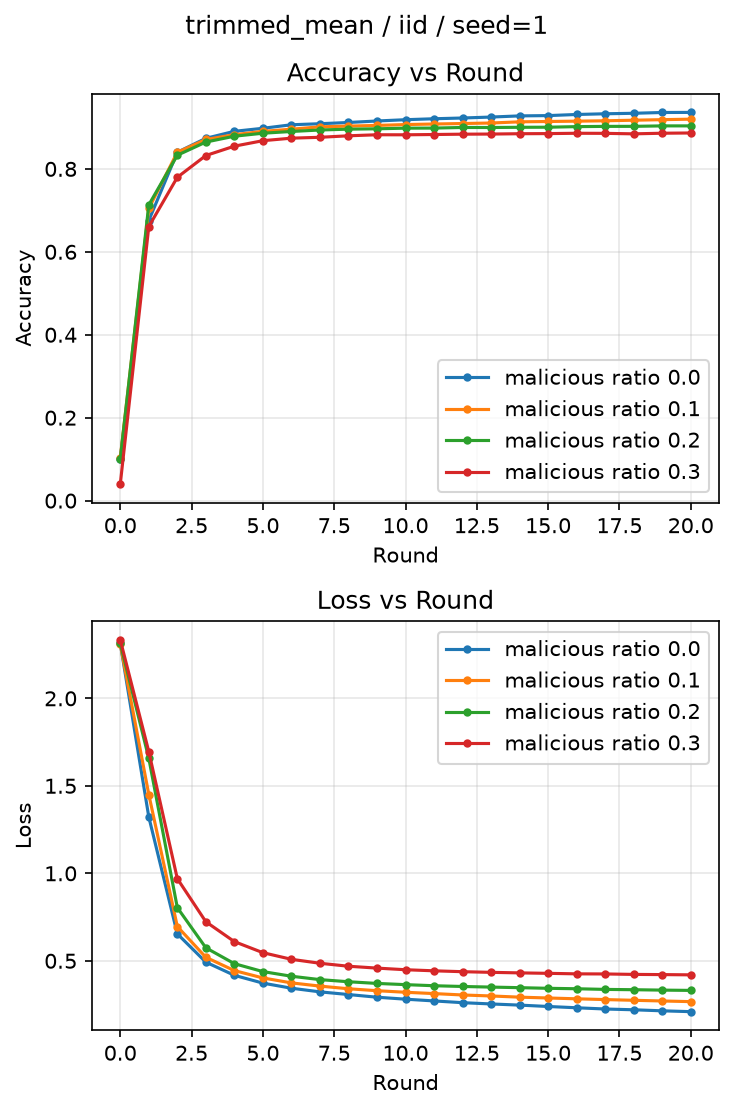
\includegraphics[width=0.85\columnwidth]{result/trimmed_mean_iid_seed1_by_ratio.png}
    \caption{Trimmed Mean・IID・Seed 1 における malicious ratio 別の Round-Accuracy および Round-Loss の推移}
    \label{fig:trimmed_mean_iid_seed1_by_ratio}
\end{figure}

\subsection{Trimmed Mean(Non-IID環境)における悪性クライアント比率別評価}
\subsubsection{実験条件}

Trimmed Meanを用いたNon-IID環境において，悪性クライアント比率を変化させ，
悪性クライアント比率がモデルの性能に与える影響を比較する．
以下の条件はすべての実験で共通とした．

\begin{itemize}
    \item \textbf{Aggregation Method：} Trimmed Mean
    \item \textbf{Data Split：} Non-IID
    \item \textbf{Attack：} Adaptive Attack
    \item \textbf{Number of Rounds：} 20
    \item \textbf{Seeds：} 1，2，3
\end{itemize}

比較対象とする悪性クライアント比率を以下に示す．

\begin{itemize}
    \item \textbf{Malicious Ratio：} 0.0，0.1，0.2，0.3
\end{itemize}

乱数の影響を考慮し，Seed値を1，2，3の3通り設定して実験を行った．
本節ではSeed 1のみの結果ではなく，Malicious Ratioごとに
Seed 1，2，3の平均値と標準偏差を算出し，平均線と標準偏差の帯を
重ねて比較する．詳細な結果（全Seedの推移）は付録に記載する．

\subsubsection{実験結果}

実験結果を図\ref{fig:trimmed_mean_noniid_seedmean_by_ratio}に示す．また，図の作成に用いたRound別のAccuracyおよびLossの数値（Seed平均$\pm$標準偏差）を付録の表\ref{tab:trimmed_mean_noniid_seedmean_by_ratio}に示す．
悪性クライアント割合0.0-0.2では,IID環境同様に収束が確認できる.
一方で,悪性クライアント割合0.3の時,収束が他の条件に比べ遅いことは自明であり,Round10付近まで緩やかに上昇を続けるうえ,標準偏差帯も広い.
これを踏まえ,Non-IID環境かつ悪性クライアント比率が高い条件でのみ,Seedに依存した不安定な挙動を示すことが確認された.
これは,Non-IID環境では座標ごとの分布形状もクライアントによって異なるため,Trimmed Meanのトリム幅を上回る割合の悪性クライアントが存在すると,
除外しきれない悪性値が座標の平均に混入しやすくなるためと考えられる.
\begin{figure}[t]
    \centering
    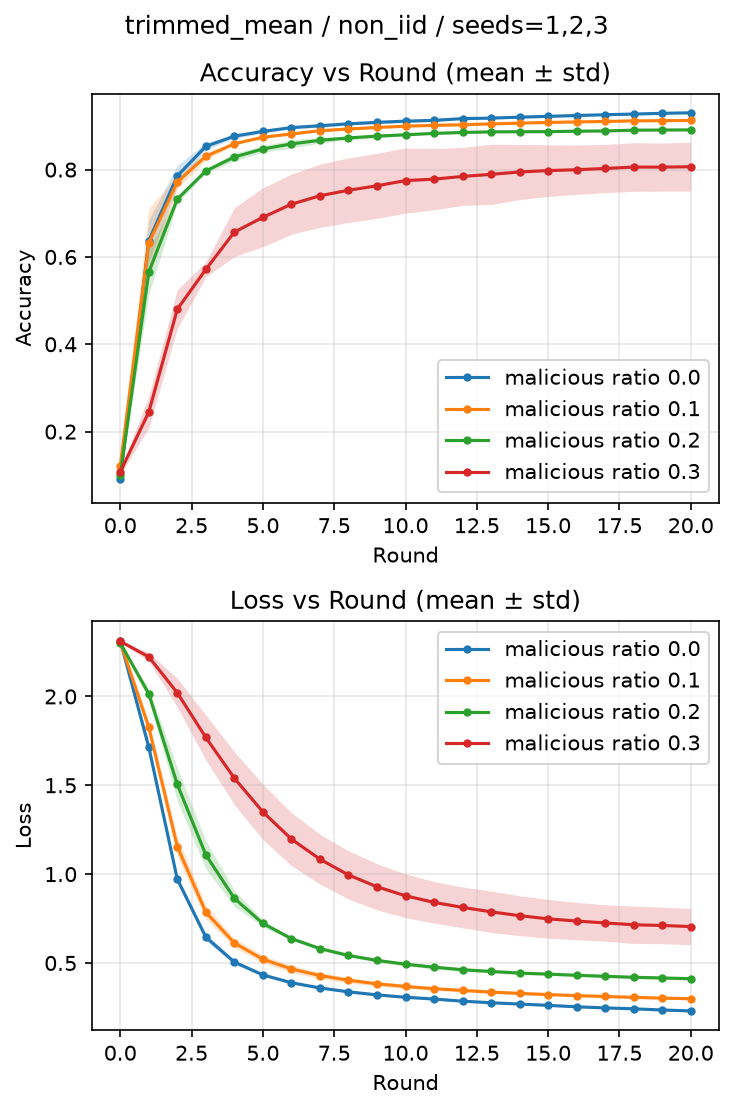
\includegraphics[width=0.85\columnwidth]{result/trimmed_mean_noniid_seedmean_by_ratio.png}
    \caption{Trimmed Mean・Non-IID における malicious ratio 別の Round-Accuracy および Round-Loss の推移（Seed 1, 2, 3 の平均 $\pm$ 標準偏差）}
    \label{fig:trimmed_mean_noniid_seedmean_by_ratio}
\end{figure}

\subsection{Krum(IID環境)における悪性クライアント比率別評価}
\subsubsection{実験条件}

Krumを用いたIID環境において，悪性クライアント比率を変化させ，
悪性クライアント比率がモデルの性能に与える影響を比較する．
以下の条件はすべての実験で共通とした．

\begin{itemize}
    \item \textbf{Aggregation Method：} Krum
    \item \textbf{Data Split：} IID
    \item \textbf{Attack：} Adaptive Attack
    \item \textbf{Number of Rounds：} 20
    \item \textbf{Seeds：} 1，2，3
\end{itemize}

比較対象とする悪性クライアント比率を以下に示す．

\begin{itemize}
    \item \textbf{Malicious Ratio：} 0.0，0.1，0.2，0.3
\end{itemize}

乱数の影響を考慮し，Seed値を1，2，3の3通り設定して実験を行った．
Krumは複数クライアントの更新を平均せず1クライアントの更新のみを
採用する集約手法であるため，本節ではSeed 1のみの結果ではなく，
Malicious Ratioごとに Seed 1，2，3（一部Roundでログが途切れたSeedを
除く）の平均値と標準偏差を算出し，平均線と標準偏差の帯を重ねて比較
する．詳細な結果（全Seedの推移）は付録に記載する．

\subsubsection{実験結果}

実験結果を図\ref{fig:krum_iid_seedmean_by_ratio}に示す．また，図の作成に用いたRound別のAccuracyおよびLossの数値（Seed平均$\pm$標準偏差）を付録の表\ref{tab:krum_iid_seedmean_by_ratio}に示す．
Malicious ratio 0.0でも収束後のAccuracyは0.87-0.93程度で細かく上下しており,Round5以降のRound間のAccuracyの変化量は0.0103と,Median,Trimmed Meanの悪性クライアント割合0.0のときの0.0026の約4倍に達する.
これはKrumが毎ラウンド1クライアントのみを選択する構造上選ばれるクライアントがラウンドごとに入れ替わることに起因すると考えられる.
悪性クライアント割合0.2,0.3ではAccuracyが学習中盤で一度ピークに達した後,終盤にかけて低下するという他の手法では見られない挙動が確認された.
この「中盤でピークに達した後に劣化する」挙動は,Adaptive Model Poisoning Attackが学習の進行に伴い悪性更新をKrumに選択されやすい形へ最適化を続けることで防御が徐々に破綻していく過程を反映していると考えられる.

\begin{figure}[t]
    \centering
    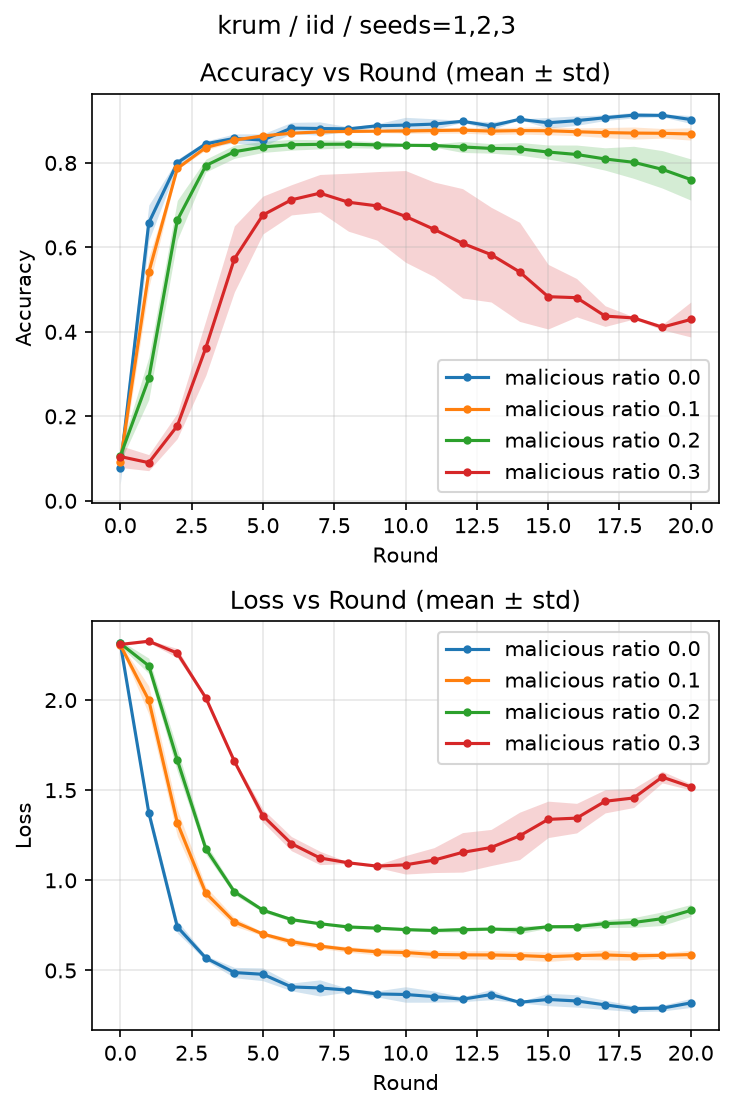
\includegraphics[width=0.85\columnwidth]{result/krum_iid_seedmean_by_ratio.png}
    \caption{Krum・IID における malicious ratio 別の Round-Accuracy および Round-Loss の推移（Seed 平均 $\pm$ 標準偏差）}
    \label{fig:krum_iid_seedmean_by_ratio}
\end{figure}

\subsection{Krum(Non-IID環境)における悪性クライアント比率別評価}
\subsubsection{実験条件}

Krumを用いたNon-IID環境において，悪性クライアント比率を変化させ，
悪性クライアント比率がモデルの性能に与える影響を比較する．
以下の条件はすべての実験で共通とした．

\begin{itemize}
    \item \textbf{Aggregation Method：} Krum
    \item \textbf{Data Split：} Non-IID
    \item \textbf{Attack：} Adaptive Attack
    \item \textbf{Number of Rounds：} 20
    \item \textbf{Seeds：} 1，2，3
\end{itemize}

比較対象とする悪性クライアント比率を以下に示す．

\begin{itemize}
    \item \textbf{Malicious Ratio：} 0.0，0.1，0.2，0.3
\end{itemize}

乱数の影響を考慮し，Seed値を1，2，3の3通り設定して実験を行った．
IID環境の場合と同様，本節でもMalicious RatioごとにSeed 1，2，3
（一部Roundでログが途切れたSeedを除く）の平均値と標準偏差を算出し，
平均線と標準偏差の帯を重ねて比較する．詳細な結果（全Seedの推移）は
付録に記載する．

\subsubsection{実験結果}

実験結果を図\ref{fig:krum_noniid_seedmean_by_ratio}に示す．また，図の作成に用いたRound別のAccuracyおよびLossの数値（Seed平均$\pm$標準偏差）を付録の表\ref{tab:krum_noniid_seedmean_by_ratio}に示す．
IID環境では良性クライアント間の分散がRound5以降ほぼ横ばいで推移するのに対し,Non-IID環境では,クライアントごとのローカルデータ分布が偏っているため,Krumが選択する少数のクライアントがラウンドごとに入れ替わるたびにモデル品質に大きく変動することが要因とされている.
悪性クライアントの割合が0.2のとき,IID環境と同様に学習中盤で0.748まで上昇した後,終盤には0.645まで低下する.割合が0.3の時,Accuracyは低迷し,収束せず,Lossも大きいことから学習が成立していないことがわかる.
以上より,KrumはNon-IID環境において,割合0.0の時点から構造的に不安定であり,割合が0.3ではAdaptive Model Poisoning Attackに対して防御がほぼ機能しないことが確認された.
\begin{figure}[t]
    \centering
    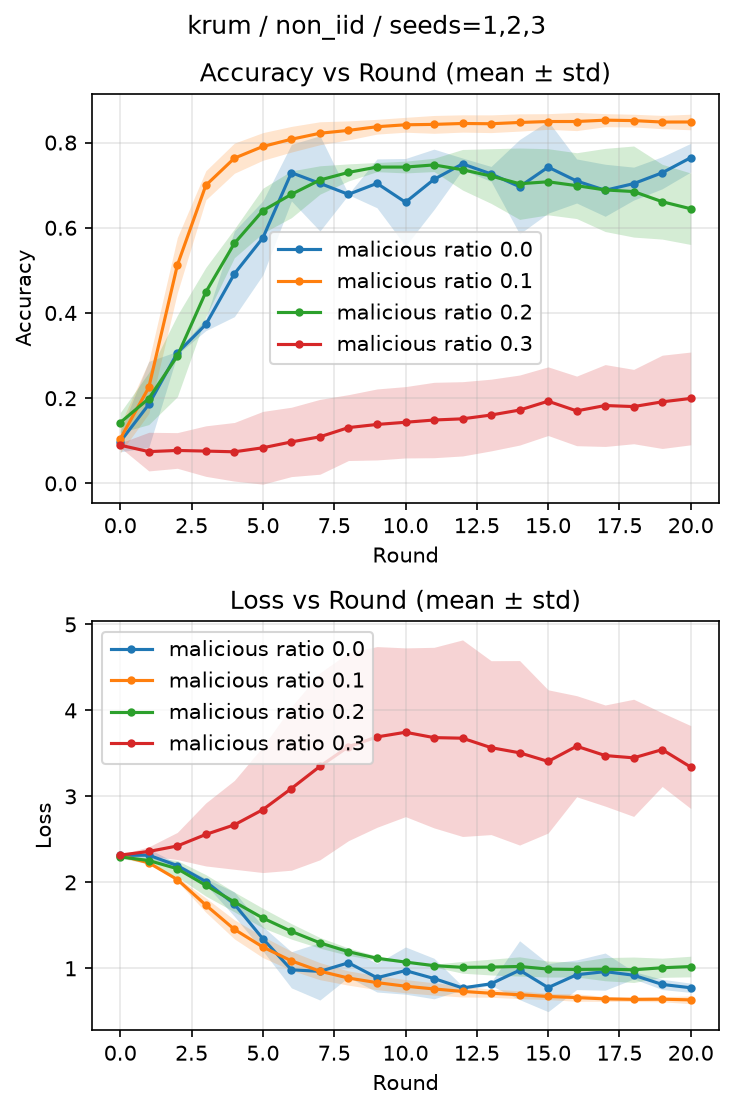
\includegraphics[width=0.85\columnwidth]{result/krum_noniid_seedmean_by_ratio.png}
    \caption{Krum・Non-IID における malicious ratio 別の Round-Accuracy および Round-Loss の推移（Seed 平均 $\pm$ 標準偏差）}
    \label{fig:krum_noniid_seedmean_by_ratio}
\end{figure}

\subsection{Bulyan(IID環境)における悪性クライアント比率別評価}
\subsubsection{実験条件}

Bulyanを用いたIID環境において，悪性クライアント比率を変化させ，
悪性クライアント比率がモデルの性能に与える影響を比較する．
以下の条件はすべての実験で共通とした．

\begin{itemize}
    \item \textbf{Aggregation Method：} Bulyan
    \item \textbf{Data Split：} IID
    \item \textbf{Attack：} Adaptive Attack
    \item \textbf{Number of Rounds：} 20
    \item \textbf{Seeds：} 1，2，3
\end{itemize}

比較対象とする悪性クライアント比率を以下に示す．

\begin{itemize}
    \item \textbf{Malicious Ratio：} 0.0，0.1，0.2
\end{itemize}

乱数の影響を考慮し，Seed値を1，2，3の3通り設定して実験を行った．
Malicious Ratio 0.3（$f=30$）はBulyanのロバスト性条件
$n \geq 4f+3$（$100 < 123$）を満たさず，Round 0以降のログが存在しない
ため，本節の比較対象から除外する．他章との表記統一のため，Malicious
RatioごとにSeed 1，2，3の平均値と標準偏差を算出し，平均線と標準偏差
の帯を重ねて比較する．詳細な結果（全Seedの推移）は付録に記載する．

\subsubsection{実験結果}

実験結果を図\ref{fig:bulyan_iid_seedmean_by_ratio}に示す．また，図の作成に用いたRound別のAccuracyおよびLossの数値（Seed平均$\pm$標準偏差）を付録の表\ref{tab:bulyan_iid_seedmean_by_ratio}に示す．
すべての悪性クライアント割合でAccuracyは振動なく単調に収束し,KrumのIID環境で見られたような中盤ピーク後の低下も見られない.最終Accuracyも割合に対する変化量が小さい.同一Ratio帯のKrum単体と比較してKrumとTrimmed Meanを合わせたBulyanは
明確に安定していることがわかる.Bulyanは複数の候補クライアントを集約した上で外れ値を除去する多段構成であるため,Krumのように単一の選択結果に依存せずIID環境では悪性クライアント割合の増加に対しても安定した挙動を維持することが確認された.
\begin{figure}[t]
    \centering
    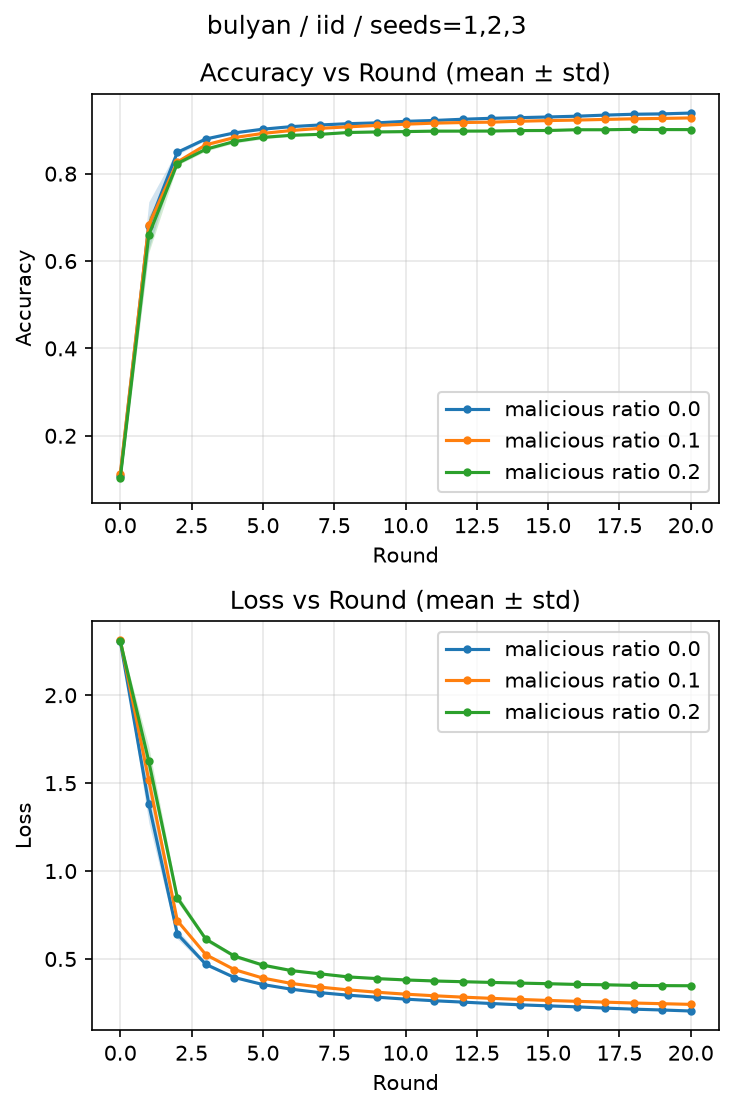
\includegraphics[width=0.85\columnwidth]{result/bulyan_iid_seedmean_by_ratio.png}
    \caption{Bulyan・IID における malicious ratio 別の Round-Accuracy および Round-Loss の推移（Seed 平均 $\pm$ 標準偏差，malicious ratio 0.3 はロバスト性条件を満たさないため対象外）}
    \label{fig:bulyan_iid_seedmean_by_ratio}
\end{figure}

\subsection{Bulyan(Non-IID環境)における悪性クライアント比率別評価}
\subsubsection{実験条件}

Bulyanを用いたNon-IID環境において，悪性クライアント比率を変化させ，
悪性クライアント比率がモデルの性能に与える影響を比較する．
以下の条件はすべての実験で共通とした．

\begin{itemize}
    \item \textbf{Aggregation Method：} Bulyan
    \item \textbf{Data Split：} Non-IID
    \item \textbf{Attack：} Adaptive Attack
    \item \textbf{Number of Rounds：} 20
    \item \textbf{Seeds：} 1，2，3
\end{itemize}

比較対象とする悪性クライアント比率を以下に示す．

\begin{itemize}
    \item \textbf{Malicious Ratio：} 0.0，0.1，0.2
\end{itemize}

乱数の影響を考慮し，Seed値を1，2，3の3通り設定して実験を行った．
IID環境の場合と同様，Malicious Ratio 0.3（$f=30$）はBulyanの
ロバスト性条件 $n \geq 4f+3$（$100 < 123$）を満たさず，Round 0以降の
ログが存在しないため，本節の比較対象から除外する．Malicious Ratio
ごとにSeed 1，2，3の平均値と標準偏差を算出し，平均線と標準偏差の帯を
重ねて比較する．詳細な結果（全Seedの推移）は付録に記載する．

\subsubsection{実験結果}

実験結果を図\ref{fig:bulyan_noniid_seedmean_by_ratio}に示す．また，図の作成に用いたRound別のAccuracyおよびLossの数値（Seed平均$\pm$標準偏差）を付録の表\ref{tab:bulyan_noniid_seedmean_by_ratio}に示す．
IID環境と同様,全ての悪性クライアント割合で振動のない滑らかな収束を示す.最終Accuracyは割合0.0と0.1で差が小さいがRatio0.2では,やや低下するし,収束もやや遅くなる.
しかしながら,同一ratio帯のKrum(Non-IID)やFedAvg(Non-IID)と比べてround間のAccuracy変化量が一桁小さい.以上より,Bulyanは実行可能なratio範囲において,Non-IID環境でも他手法より高い安定性を維持するが,
Ratio0.2で標準偏差が拡大し始めている点は，ロバスト性条件の上限（Ratio 0.25 で $n < 4f+3$）に近づくにつれて余裕が減少していることを示唆している．
\begin{figure}[t]
    \centering
    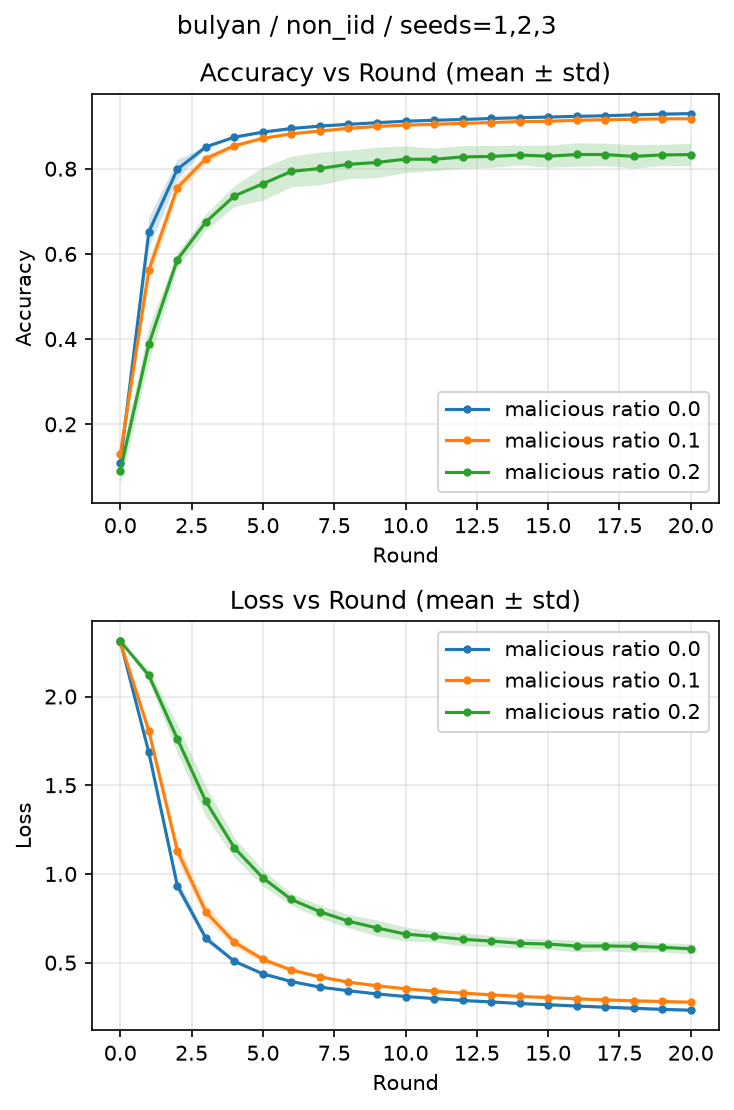
\includegraphics[width=0.85\columnwidth]{result/bulyan_noniid_seedmean_by_ratio.png}
    \caption{Bulyan・Non-IID における malicious ratio 別の Round-Accuracy および Round-Loss の推移（Seed 平均 $\pm$ 標準偏差，malicious ratio 0.3 はロバスト性条件を満たさないため対象外）}
    \label{fig:bulyan_noniid_seedmean_by_ratio}
\end{figure}

\section{全体的な結論と考察}

本研究では，MNISTを用いたFederated Learning環境において，FedAvg，Median，Trimmed Mean，Krum，Bulyanの5種類の集約手法に対しAdaptive Model Poisoning Attackを適用し，IID環境およびNon-IID環境における耐性を評価した．

外れ値を除外する仕組みを持たないFedAvgは，悪性クライアント割合が0.2以上になるとAccuracyが大きく低下し，0.3では学習が崩壊することが確認された．一方，MedianおよびTrimmed Meanは，検証した悪性クライアント割合の範囲においてSeed間のばらつきも小さく，比較的ロバストな挙動を示した．ただし，Non-IID環境かつ悪性クライアント割合が高い条件（Trimmed Mean，Ratio 0.3）では，座標ごとのトリム幅を上回る悪性クライアントが存在するために除外しきれない悪性値が平均へ混入し，収束が他の条件と比べ遅延する傾向が見られた．

Krumは，Malicious Ratio 0.0の時点でもラウンドごとに選択されるクライアントが入れ替わるためAccuracyの変動が他手法より大きく，悪性クライアント割合が0.2以上になると学習中盤でAccuracyが一度ピークに達した後に低下するという，他の手法では見られない挙動を示した．これは，Adaptive Model Poisoning Attackが学習の進行に伴い悪性更新をKrumに選択されやすい形へ最適化を続けることで，防御が徐々に破綻していく過程を反映していると考えられる．特にNon-IID環境のKrumは，悪性クライアント割合0.3において学習がほぼ成立しなくなることが確認された．

BulyanはKrumによる候補選択とTrimmed Meanによる集約を組み合わせているため，Krum単体と比較して振動が少なく，悪性クライアント割合の増加に対しても安定した収束を示した．ただし，ロバスト性条件$n \geq 4f+3$の制約により，本実験の設定（$n=100$）ではMalicious Ratio 0.3（$f=30$）を評価できず，比較可能な範囲はRatio 0.2までにとどまった．

以上より，Fangらが論文「Local Model Poisoning Attacks to Byzantine-Robust Federated Learning」で指摘している

\begin{enumerate}
    \item 攻撃者が増えるほど精度が悪化する点
    \item Non-IID環境はIID環境に比べ精度が悪化する点
    \item 手法の中でKrumが最も弱い点
\end{enumerate}

の3点を，本実験でも一貫して確認することができた．

一方で，本実験ではSeed数を3に限定して評価を行っており，各章の実験結果でも述べた通り，特にKrumやFedAvgのNon-IID環境かつ悪性クライアント割合が高い条件では，Seed間で最終Accuracyや収束の傾向に無視できないばらつきが見られた．そのため，現時点で得られた「ロバスト性の強弱」の傾向は，Seed数を増やした上で統計的な安定性を検証する必要があり，今後の課題としたい．また，本実装はFangらの数式をそのまま再現したものではなく近似・簡略化した再実装であるため，攻撃がどのような機構で防御を回避しているのかについても，更新ベクトルの距離構造などに基づいた定量的な分析を通じて明らかにしていく必要がある．


































































































\begin{thebibliography}{99}

\bibitem{mammen2021fl}
Priyanka Mary Mammen,
``Federated Learning: Opportunities and Challenges,''
Proceedings of ACM Conference,
2021.
\bibitem{li2019fl}
Tian Li,
Anit Kumar Sahu,
Ameet Talwalkar,
Virginia Smith,
``Federated Learning: Challenges, Methods, and Future Directions,''
arXiv preprint arXiv:1908.07873,
2019.
\bibitem{ma2020privacy}
Chuan Ma,
Jun Li,
Ming Ding,
Howard H. Yang,
Feng Shu,
Tony Q. S. Quek,
H. Vincent Poor,
``On Safeguarding Privacy and Security in the Framework of Federated Learning,''
arXiv preprint arXiv:1909.06512,
2020.

\bibitem{sagar2023survey}
Subhash Sagar,
Chang-Tsun Li,
Seng W. Loke,
Jinho Choi,
``Poisoning Attacks and Defenses in Federated Learning: A Survey,''
IEEE Security \& Privacy,
2023.

\bibitem{fang2020local}
Minghong Fang,
Xiaoyu Cao,
Jinyuan Jia,
Neil Zhenqiang Gong,
``Local Model Poisoning Attacks to Byzantine-Robust Federated Learning,''
Proceedings of the 29th USENIX Security Symposium (USENIX Security 2020),
pp. 1605--1622,
2020.
\bibitem{mcmahan2017fedavg}
H. Brendan McMahan,
Eider Moore,
Daniel Ramage,
Seth Hampson,
Blaise Aguera y Arcas,
``Communication-Efficient Learning of Deep Networks from Decentralized Data,''
Proceedings of the 20th International Conference on Artificial Intelligence and Statistics (AISTATS),
pp. 1273--1282,
2017.
\bibitem{xie2020dba}
Chulin Xie,
Keli Huang,
Pin-Yu Chen,
Bo Li,
``DBA: Distributed Backdoor Attacks against Federated Learning,''
International Conference on Learning Representations (ICLR),
2020.
\bibitem{nguyen2022flame}
Tuan D. Nguyen et al.,
``FLAME: Taming Backdoors in Federated Learning,''
31st USENIX Security Symposium (USENIX Security 2022),
pp. 1415--1432,
2022.
\bibitem{bagdasaryan2020model}
Eugene Bagdasaryan,
Andreas Veit,
Yiqing Hua,
Deborah Estrin,
Vitaly Shmatikov,
``How To Backdoor Federated Learning,''
Proceedings of the 23rd International Conference on Artificial Intelligence and Statistics (AISTATS),
pp. 2938--2948,
2020.
\end{thebibliography}

\clearpage
\onecolumn

\section{付録}
「result.csv」にデータがあります.
\begin{table}[H]
\centering
\caption{FedAvg・IID・Seed 1 における malicious ratio 別の Round-Accuracy と Round-Loss}
\label{tab:fedavg_iid_seed1_by_ratio}

\footnotesize
\setlength{\tabcolsep}{4pt}
\renewcommand{\arraystretch}{0.90}

\begin{tabular}{c cc cc cc cc}

\toprule

& \multicolumn{2}{c}{Ratio 0.0}
& \multicolumn{2}{c}{Ratio 0.1}
& \multicolumn{2}{c}{Ratio 0.2}
& \multicolumn{2}{c}{Ratio 0.3} \\

\cmidrule(lr){2-3}
\cmidrule(lr){4-5}
\cmidrule(lr){6-7}
\cmidrule(lr){8-9}

Round
& Acc. & Loss
& Acc. & Loss
& Acc. & Loss
& Acc. & Loss \\

\midrule

0 & 0.1416 & 2.2942 & 0.1008 & 2.3051 & 0.0778 & 2.3114 & 0.1050 & 2.3052 \\
1 & 0.7636 & 1.2828 & 0.7395 & 0.8810 & 0.6285 & 1.2967 & 0.4669 & 2.4719 \\
2 & 0.8531 & 0.6233 & 0.8484 & 0.5087 & 0.5945 & 1.0478 & 0.4176 & 5.5211 \\
3 & 0.8811 & 0.4643 & 0.8869 & 0.4138 & 0.6020 & 1.4075 & 0.2155 & 16.0470 \\
4 & 0.8948 & 0.3896 & 0.8944 & 0.3540 & 0.2978 & 4.8879 & 0.1950 & 9.2702 \\
5 & 0.9038 & 0.3488 & 0.9095 & 0.3165 & 0.3474 & 4.0723 & 0.3092 & 2.0615 \\
6 & 0.9081 & 0.3229 & 0.9089 & 0.3013 & 0.3068 & 3.8003 & 0.4707 & 3.5233 \\
7 & 0.9136 & 0.3033 & 0.9205 & 0.2748 & 0.4908 & 3.1571 & 0.2986 & 6.2982 \\
8 & 0.9156 & 0.2891 & 0.9213 & 0.2616 & 0.2649 & 5.8880 & 0.3447 & 8.0512 \\
9 & 0.9180 & 0.2761 & 0.9270 & 0.2465 & 0.2661 & 10.8871 & 0.3933 & 7.0966 \\
10 & 0.9206 & 0.2655 & 0.9306 & 0.2371 & 0.4560 & 5.0990 & 0.5659 & 1.5118 \\
11 & 0.9223 & 0.2569 & 0.9289 & 0.2352 & 0.3958 & 5.1416 & 0.3522 & 5.3616 \\
12 & 0.9254 & 0.2476 & 0.9354 & 0.2202 & 0.6644 & 2.4425 & 0.4672 & 5.4911 \\
13 & 0.9271 & 0.2409 & 0.9361 & 0.2104 & 0.6441 & 1.3076 & 0.5873 & 2.3319 \\
14 & 0.9283 & 0.2336 & 0.9382 & 0.2047 & 0.6269 & 2.1362 & 0.4728 & 2.9704 \\
15 & 0.9301 & 0.2268 & 0.9368 & 0.2039 & 0.3989 & 4.6093 & 0.4600 & 2.3754 \\
16 & 0.9322 & 0.2200 & 0.9403 & 0.1972 & 0.4244 & 4.0273 & 0.6398 & 2.2465 \\
17 & 0.9331 & 0.2138 & 0.9404 & 0.1996 & 0.5916 & 1.8398 & 0.5357 & 2.4792 \\
18 & 0.9355 & 0.2074 & 0.9414 & 0.2013 & 0.6079 & 2.0978 & 0.5437 & 3.8618 \\
19 & 0.9380 & 0.2027 & 0.9346 & 0.2194 & 0.6875 & 2.0099 & 0.4995 & 3.6105 \\
20 & 0.9382 & 0.1989 & 0.9367 & 0.2168 & 0.5231 & 3.5254 & 0.6567 & 1.8212 \\

\bottomrule

\end{tabular}

\end{table}

\begin{table}[H]
\centering
\caption{FedAvg・IID・Seed 2 における malicious ratio 別の Round-Accuracy と Round-Loss}
\label{tab:fedavg_iid_seed2_by_ratio}

\footnotesize
\setlength{\tabcolsep}{4pt}
\renewcommand{\arraystretch}{0.90}

\begin{tabular}{c cc cc cc cc}

\toprule

& \multicolumn{2}{c}{Ratio 0.0}
& \multicolumn{2}{c}{Ratio 0.1}
& \multicolumn{2}{c}{Ratio 0.2}
& \multicolumn{2}{c}{Ratio 0.3} \\

\cmidrule(lr){2-3}
\cmidrule(lr){4-5}
\cmidrule(lr){6-7}
\cmidrule(lr){8-9}

Round
& Acc. & Loss
& Acc. & Loss
& Acc. & Loss
& Acc. & Loss \\

\midrule

0 & 0.0975 & 2.2943 & 0.0817 & 2.3042 & 0.0869 & 2.2993 & 0.0871 & 2.3058 \\
1 & 0.7217 & 1.2678 & 0.6801 & 0.9412 & 0.6540 & 1.1425 & 0.6494 & 2.0048 \\
2 & 0.8399 & 0.6505 & 0.8372 & 0.5310 & 0.6856 & 0.8765 & 0.1258 & 7.9264 \\
3 & 0.8725 & 0.4871 & 0.8806 & 0.4062 & 0.6622 & 1.0375 & 0.2638 & 11.3932 \\
4 & 0.8869 & 0.4124 & 0.8947 & 0.3543 & 0.5780 & 1.9192 & 0.1685 & 9.0113 \\
5 & 0.8957 & 0.3697 & 0.9112 & 0.3099 & 0.2637 & 5.5046 & 0.2908 & 4.2999 \\
6 & 0.9006 & 0.3415 & 0.9053 & 0.3030 & 0.4028 & 5.4084 & 0.3120 & 4.1903 \\
7 & 0.9049 & 0.3221 & 0.9209 & 0.2693 & 0.3910 & 3.8948 & 0.3903 & 3.1011 \\
8 & 0.9096 & 0.3036 & 0.9207 & 0.2593 & 0.3611 & 2.6517 & 0.2819 & 5.5339 \\
9 & 0.9128 & 0.2904 & 0.9251 & 0.2522 & 0.4259 & 3.3033 & 0.4275 & 2.8813 \\
10 & 0.9156 & 0.2783 & 0.9272 & 0.2394 & 0.4990 & 3.8053 & 0.3882 & 5.0619 \\
11 & 0.9200 & 0.2674 & 0.9347 & 0.2224 & 0.5100 & 1.6177 & 0.4414 & 3.9600 \\
12 & 0.9214 & 0.2591 & 0.9370 & 0.2110 & 0.5892 & 2.0458 & 0.5925 & 1.6918 \\
13 & 0.9236 & 0.2504 & 0.9411 & 0.2026 & 0.5014 & 3.6747 & 0.4998 & 2.7261 \\
14 & 0.9263 & 0.2419 & 0.9404 & 0.1990 & 0.5885 & 1.9194 & 0.4132 & 4.2478 \\
15 & 0.9284 & 0.2351 & 0.9419 & 0.1948 & 0.5156 & 2.7631 & 0.4168 & 6.8800 \\
16 & 0.9299 & 0.2285 & 0.9425 & 0.1871 & 0.5385 & 3.1985 & 0.4692 & 2.6400 \\
17 & 0.9336 & 0.2203 & 0.9439 & 0.1872 & 0.5363 & 3.2618 & 0.2809 & 5.1705 \\
18 & 0.9359 & 0.2146 & 0.9420 & 0.1907 & 0.3399 & 5.3854 & 0.4397 & 3.6397 \\
19 & 0.9362 & 0.2090 & 0.9443 & 0.1869 & 0.5631 & 4.8583 & 0.4574 & 6.9452 \\
20 & 0.9383 & 0.2040 & 0.9418 & 0.1920 & 0.4904 & 3.4841 & 0.5257 & 6.6401 \\

\bottomrule

\end{tabular}

\end{table}

\begin{table}[H]
\centering
\caption{FedAvg・IID・Seed 3 における malicious ratio 別の Round-Accuracy と Round-Loss}
\label{tab:fedavg_iid_seed3_by_ratio}

\footnotesize
\setlength{\tabcolsep}{4pt}
\renewcommand{\arraystretch}{0.90}

\begin{tabular}{c cc cc cc cc}

\toprule

& \multicolumn{2}{c}{Ratio 0.0}
& \multicolumn{2}{c}{Ratio 0.1}
& \multicolumn{2}{c}{Ratio 0.2}
& \multicolumn{2}{c}{Ratio 0.3} \\

\cmidrule(lr){2-3}
\cmidrule(lr){4-5}
\cmidrule(lr){6-7}
\cmidrule(lr){8-9}

Round
& Acc. & Loss
& Acc. & Loss
& Acc. & Loss
& Acc. & Loss \\

\midrule

0 & 0.0877 & 2.3024 & 0.0608 & 2.3152 & 0.0844 & 2.3129 & 0.1121 & 2.3028 \\
1 & 0.7259 & 1.2749 & 0.7056 & 0.9331 & 0.5934 & 1.3403 & 0.6388 & 1.6048 \\
2 & 0.8336 & 0.6461 & 0.8329 & 0.5351 & 0.5800 & 1.3043 & 0.3630 & 3.5062 \\
3 & 0.8694 & 0.5020 & 0.8808 & 0.4107 & 0.6616 & 1.1254 & 0.2382 & 9.7461 \\
4 & 0.8851 & 0.4265 & 0.8931 & 0.3396 & 0.3567 & 4.1239 & 0.0982 & 17.7718 \\
5 & 0.8970 & 0.3782 & 0.9093 & 0.3112 & 0.4327 & 3.6166 & 0.1831 & 12.4552 \\
6 & 0.9037 & 0.3449 & 0.9105 & 0.2889 & 0.3408 & 2.7942 & 0.0986 & 12.0350 \\
7 & 0.9102 & 0.3213 & 0.9126 & 0.2854 & 0.4221 & 4.8563 & 0.4063 & 7.4052 \\
8 & 0.9136 & 0.3040 & 0.9210 & 0.2582 & 0.2987 & 8.1121 & 0.3436 & 5.2857 \\
9 & 0.9156 & 0.2909 & 0.9261 & 0.2421 & 0.4264 & 5.5301 & 0.4488 & 3.4722 \\
10 & 0.9182 & 0.2785 & 0.9304 & 0.2305 & 0.4844 & 4.8675 & 0.2295 & 6.4546 \\
11 & 0.9212 & 0.2675 & 0.9352 & 0.2144 & 0.5771 & 2.6495 & 0.4053 & 4.2804 \\
12 & 0.9236 & 0.2588 & 0.9344 & 0.2174 & 0.4898 & 2.6568 & 0.3749 & 4.3466 \\
13 & 0.9256 & 0.2504 & 0.9398 & 0.1976 & 0.4291 & 3.6676 & 0.5469 & 3.3843 \\
14 & 0.9286 & 0.2425 & 0.9369 & 0.2061 & 0.4700 & 3.1586 & 0.5318 & 2.5925 \\
15 & 0.9300 & 0.2356 & 0.9419 & 0.1871 & 0.5194 & 3.6085 & 0.3739 & 4.1574 \\
16 & 0.9308 & 0.2300 & 0.9389 & 0.2025 & 0.6054 & 2.3273 & 0.5030 & 4.6876 \\
17 & 0.9322 & 0.2229 & 0.9419 & 0.1864 & 0.5940 & 1.9801 & 0.5539 & 2.4600 \\
18 & 0.9339 & 0.2173 & 0.9369 & 0.2140 & 0.6257 & 1.9355 & 0.5016 & 3.6686 \\
19 & 0.9352 & 0.2111 & 0.9381 & 0.1956 & 0.5236 & 3.0180 & 0.6246 & 2.2948 \\
20 & 0.9368 & 0.2071 & 0.9299 & 0.2462 & 0.6422 & 1.5237 & 0.5313 & 2.3416 \\

\bottomrule

\end{tabular}

\end{table}

\begin{table}[H]
\centering
\caption{FedAvg・Non-IID・Seed 1 における malicious ratio 別の Round-Accuracy と Round-Loss}
\label{tab:fedavg_noniid_seed1_by_ratio}

\footnotesize
\setlength{\tabcolsep}{4pt}
\renewcommand{\arraystretch}{0.90}

\begin{tabular}{c cc cc cc cc}

\toprule

& \multicolumn{2}{c}{Ratio 0.0}
& \multicolumn{2}{c}{Ratio 0.1}
& \multicolumn{2}{c}{Ratio 0.2}
& \multicolumn{2}{c}{Ratio 0.3} \\

\cmidrule(lr){2-3}
\cmidrule(lr){4-5}
\cmidrule(lr){6-7}
\cmidrule(lr){8-9}

Round
& Acc. & Loss
& Acc. & Loss
& Acc. & Loss
& Acc. & Loss \\

\midrule

0 & 0.1309 & 2.3044 & 0.0888 & 2.3117 & 0.0973 & 2.3204 & 0.1034 & 2.3123 \\
1 & 0.6813 & 1.5418 & 0.4907 & 1.4176 & 0.5410 & 1.5413 & 0.3943 & 4.0645 \\
2 & 0.8172 & 0.8180 & 0.7903 & 0.6440 & 0.5934 & 1.3894 & 0.2932 & 6.0693 \\
3 & 0.8601 & 0.5698 & 0.8068 & 0.6132 & 0.5378 & 2.5099 & 0.3721 & 7.7834 \\
4 & 0.8831 & 0.4568 & 0.8762 & 0.4067 & 0.2775 & 3.6061 & 0.1160 & 4.3092 \\
5 & 0.8934 & 0.3930 & 0.8532 & 0.4731 & 0.5220 & 2.6530 & 0.3485 & 4.6312 \\
6 & 0.9004 & 0.3579 & 0.8952 & 0.3309 & 0.3476 & 1.9810 & 0.1480 & 11.2444 \\
7 & 0.9065 & 0.3314 & 0.8750 & 0.4112 & 0.5902 & 2.4553 & 0.2205 & 8.1592 \\
8 & 0.9081 & 0.3153 & 0.9118 & 0.2813 & 0.3308 & 3.0394 & 0.3376 & 4.2791 \\
9 & 0.9125 & 0.3000 & 0.9073 & 0.3085 & 0.5940 & 2.4173 & 0.2795 & 5.6537 \\
10 & 0.9146 & 0.2872 & 0.9232 & 0.2505 & 0.5829 & 1.7733 & 0.3352 & 4.6932 \\
11 & 0.9182 & 0.2766 & 0.9226 & 0.2639 & 0.5622 & 2.6095 & 0.2480 & 8.2213 \\
12 & 0.9182 & 0.2678 & 0.9278 & 0.2372 & 0.6217 & 2.6759 & 0.3622 & 4.4483 \\
13 & 0.9220 & 0.2597 & 0.9266 & 0.2440 & 0.6387 & 1.8780 & 0.3161 & 6.3737 \\
14 & 0.9251 & 0.2506 & 0.9345 & 0.2156 & 0.5614 & 2.2875 & 0.3647 & 3.5018 \\
15 & 0.9263 & 0.2451 & 0.9338 & 0.2176 & 0.5870 & 2.6185 & 0.5519 & 2.2887 \\
16 & 0.9282 & 0.2379 & 0.9370 & 0.2101 & 0.6694 & 1.3393 & 0.4549 & 2.3835 \\
17 & 0.9301 & 0.2300 & 0.9369 & 0.2048 & 0.5571 & 2.2798 & 0.6099 & 1.5903 \\
18 & 0.9322 & 0.2245 & 0.9368 & 0.2045 & 0.7287 & 1.5247 & 0.4438 & 3.1132 \\
19 & 0.9344 & 0.2186 & 0.9404 & 0.1903 & 0.5659 & 2.4085 & 0.6115 & 2.2956 \\
20 & 0.9358 & 0.2139 & 0.9407 & 0.1938 & 0.7097 & 1.5180 & 0.6216 & 1.7027 \\

\bottomrule

\end{tabular}

\end{table}

\begin{table}[H]
\centering
\caption{FedAvg・Non-IID・Seed 2 における malicious ratio 別の Round-Accuracy と Round-Loss}
\label{tab:fedavg_noniid_seed2_by_ratio}

\footnotesize
\setlength{\tabcolsep}{4pt}
\renewcommand{\arraystretch}{0.90}

\begin{tabular}{c cc cc cc cc}

\toprule

& \multicolumn{2}{c}{Ratio 0.0}
& \multicolumn{2}{c}{Ratio 0.1}
& \multicolumn{2}{c}{Ratio 0.2}
& \multicolumn{2}{c}{Ratio 0.3} \\

\cmidrule(lr){2-3}
\cmidrule(lr){4-5}
\cmidrule(lr){6-7}
\cmidrule(lr){8-9}

Round
& Acc. & Loss
& Acc. & Loss
& Acc. & Loss
& Acc. & Loss \\

\midrule

0 & 0.0551 & 2.3235 & 0.0956 & 2.3107 & 0.0638 & 2.3094 & 0.0836 & 2.3063 \\
1 & 0.7461 & 1.5430 & 0.5263 & 1.3088 & 0.4984 & 1.6995 & 0.5550 & 1.5304 \\
2 & 0.8381 & 0.7929 & 0.7408 & 0.7405 & 0.6984 & 1.0449 & 0.4004 & 2.5366 \\
3 & 0.8711 & 0.5429 & 0.7298 & 0.7646 & 0.4184 & 2.4602 & 0.3604 & 4.8719 \\
4 & 0.8886 & 0.4391 & 0.7494 & 0.6993 & 0.4709 & 2.4167 & 0.4559 & 2.7775 \\
5 & 0.8964 & 0.3878 & 0.7250 & 0.8406 & 0.2893 & 4.9162 & 0.3804 & 3.5787 \\
6 & 0.9023 & 0.3531 & 0.6832 & 0.9045 & 0.4977 & 2.2910 & 0.3995 & 4.6855 \\
7 & 0.9064 & 0.3291 & 0.7147 & 0.9640 & 0.3096 & 3.7268 & 0.3541 & 3.2808 \\
8 & 0.9097 & 0.3114 & 0.6961 & 0.8878 & 0.3922 & 4.0428 & 0.4989 & 2.0967 \\
9 & 0.9144 & 0.2957 & 0.7339 & 0.9507 & 0.4561 & 2.9964 & 0.3428 & 3.3955 \\
10 & 0.9153 & 0.2870 & 0.7600 & 0.7094 & 0.6216 & 1.3719 & 0.4936 & 4.3062 \\
11 & 0.9200 & 0.2753 & 0.7862 & 0.7605 & 0.5309 & 2.7498 & 0.4815 & 2.2636 \\
12 & 0.9224 & 0.2651 & 0.7814 & 0.6721 & 0.5416 & 2.2559 & 0.5710 & 1.8981 \\
13 & 0.9244 & 0.2567 & 0.7987 & 0.7292 & 0.5389 & 2.6607 & 0.5548 & 1.8491 \\
14 & 0.9252 & 0.2489 & 0.7965 & 0.6483 & 0.5124 & 2.2549 & 0.6394 & 2.1268 \\
15 & 0.9283 & 0.2420 & 0.7889 & 0.7851 & 0.5629 & 2.6167 & 0.5757 & 2.2955 \\
16 & 0.9302 & 0.2340 & 0.7992 & 0.6833 & 0.6023 & 1.6619 & 0.5864 & 2.2994 \\
17 & 0.9321 & 0.2270 & 0.7883 & 0.7947 & 0.5506 & 2.4055 & 0.5535 & 2.5547 \\
18 & 0.9324 & 0.2218 & 0.7898 & 0.7746 & 0.6948 & 1.5097 & 0.5436 & 4.0696 \\
19 & 0.9339 & 0.2151 & 0.8333 & 0.6385 & 0.6261 & 1.5921 & 0.5929 & 3.1858 \\
20 & 0.9360 & 0.2101 & 0.8391 & 0.6121 & 0.7113 & 1.3562 & 0.6610 & 1.2175 \\

\bottomrule

\end{tabular}

\end{table}

\begin{table}[H]
\centering
\caption{FedAvg・Non-IID・Seed 3 における malicious ratio 別の Round-Accuracy と Round-Loss}
\label{tab:fedavg_noniid_seed3_by_ratio}

\footnotesize
\setlength{\tabcolsep}{4pt}
\renewcommand{\arraystretch}{0.90}

\begin{tabular}{c cc cc cc cc}

\toprule

& \multicolumn{2}{c}{Ratio 0.0}
& \multicolumn{2}{c}{Ratio 0.1}
& \multicolumn{2}{c}{Ratio 0.2}
& \multicolumn{2}{c}{Ratio 0.3} \\

\cmidrule(lr){2-3}
\cmidrule(lr){4-5}
\cmidrule(lr){6-7}
\cmidrule(lr){8-9}

Round
& Acc. & Loss
& Acc. & Loss
& Acc. & Loss
& Acc. & Loss \\

\midrule

0 & 0.0757 & 2.3088 & 0.1141 & 2.2973 & 0.0991 & 2.3226 & 0.0881 & 2.3241 \\
1 & 0.6530 & 1.6055 & 0.5860 & 1.3126 & 0.5714 & 1.2292 & 0.4735 & 2.4689 \\
2 & 0.8122 & 0.8387 & 0.8314 & 0.5615 & 0.6353 & 1.1932 & 0.1742 & 4.8393 \\
3 & 0.8674 & 0.5688 & 0.8135 & 0.5911 & 0.4155 & 2.6081 & 0.2344 & 11.2079 \\
4 & 0.8829 & 0.4576 & 0.8856 & 0.3946 & 0.3382 & 3.5149 & 0.1945 & 9.4070 \\
5 & 0.8920 & 0.3995 & 0.8468 & 0.5037 & 0.2979 & 2.6513 & 0.3168 & 4.3471 \\
6 & 0.9016 & 0.3617 & 0.8963 & 0.3408 & 0.5951 & 2.1735 & 0.3771 & 3.0063 \\
7 & 0.9054 & 0.3395 & 0.8494 & 0.4967 & 0.1992 & 6.5454 & 0.4030 & 4.8088 \\
8 & 0.9076 & 0.3201 & 0.8941 & 0.3333 & 0.5332 & 4.3001 & 0.3055 & 9.2578 \\
9 & 0.9109 & 0.3065 & 0.8517 & 0.5064 & 0.5326 & 2.3781 & 0.3053 & 3.8743 \\
10 & 0.9140 & 0.2953 & 0.8898 & 0.3373 & 0.4945 & 3.6104 & 0.5073 & 1.8854 \\
11 & 0.9171 & 0.2837 & 0.8440 & 0.5517 & 0.4640 & 3.1000 & 0.5497 & 1.9574 \\
12 & 0.9186 & 0.2739 & 0.8879 & 0.3355 & 0.4951 & 2.3435 & 0.5874 & 2.0402 \\
13 & 0.9209 & 0.2656 & 0.8483 & 0.5222 & 0.4315 & 4.7904 & 0.5214 & 2.0547 \\
14 & 0.9238 & 0.2572 & 0.8893 & 0.3314 & 0.6290 & 2.4926 & 0.6349 & 1.7163 \\
15 & 0.9253 & 0.2503 & 0.8475 & 0.5202 & 0.5226 & 1.9718 & 0.5764 & 1.5382 \\
16 & 0.9262 & 0.2434 & 0.8794 & 0.3563 & 0.6477 & 1.5631 & 0.5705 & 2.5396 \\
17 & 0.9290 & 0.2357 & 0.8448 & 0.5332 & 0.6615 & 1.5053 & 0.5826 & 2.3054 \\
18 & 0.9303 & 0.2284 & 0.8722 & 0.3961 & 0.6122 & 1.8498 & 0.4358 & 3.2613 \\
19 & 0.9318 & 0.2232 & 0.8187 & 0.6207 & 0.6393 & 2.5925 & 0.4910 & 5.4931 \\
20 & 0.9329 & 0.2178 & 0.8574 & 0.4563 & 0.6039 & 1.7788 & 0.7119 & 1.6772 \\

\bottomrule

\end{tabular}

\end{table}

\begin{table}[H]
\centering
\caption{Median・IID・Seed 1 における malicious ratio 別の Round-Accuracy と Round-Loss}
\label{tab:median_iid_seed1_by_ratio}

\footnotesize
\setlength{\tabcolsep}{4pt}
\renewcommand{\arraystretch}{0.90}

\begin{tabular}{c cc cc cc cc}

\toprule

& \multicolumn{2}{c}{Ratio 0.0}
& \multicolumn{2}{c}{Ratio 0.1}
& \multicolumn{2}{c}{Ratio 0.2}
& \multicolumn{2}{c}{Ratio 0.3} \\

\cmidrule(lr){2-3}
\cmidrule(lr){4-5}
\cmidrule(lr){6-7}
\cmidrule(lr){8-9}

Round
& Acc. & Loss
& Acc. & Loss
& Acc. & Loss
& Acc. & Loss \\

\midrule

0 & 0.0920 & 2.3222 & 0.0864 & 2.3117 & 0.1052 & 2.3015 & 0.0800 & 2.3165 \\
1 & 0.6707 & 1.3895 & 0.7043 & 1.4725 & 0.7361 & 1.4644 & 0.6250 & 1.7308 \\
2 & 0.8524 & 0.6531 & 0.8397 & 0.7079 & 0.8356 & 0.7316 & 0.8050 & 0.9383 \\
3 & 0.8798 & 0.4794 & 0.8711 & 0.5224 & 0.8623 & 0.5486 & 0.8509 & 0.6628 \\
4 & 0.8915 & 0.4026 & 0.8870 & 0.4385 & 0.8773 & 0.4716 & 0.8694 & 0.5526 \\
5 & 0.8998 & 0.3609 & 0.8942 & 0.3918 & 0.8884 & 0.4279 & 0.8766 & 0.4956 \\
6 & 0.9073 & 0.3321 & 0.8990 & 0.3639 & 0.8919 & 0.4005 & 0.8835 & 0.4619 \\
7 & 0.9116 & 0.3121 & 0.9038 & 0.3436 & 0.8944 & 0.3810 & 0.8872 & 0.4405 \\
8 & 0.9148 & 0.2963 & 0.9070 & 0.3284 & 0.8971 & 0.3675 & 0.8893 & 0.4251 \\
9 & 0.9175 & 0.2848 & 0.9091 & 0.3164 & 0.8984 & 0.3561 & 0.8900 & 0.4146 \\
10 & 0.9192 & 0.2748 & 0.9117 & 0.3069 & 0.9005 & 0.3473 & 0.8899 & 0.4084 \\
11 & 0.9210 & 0.2650 & 0.9126 & 0.2982 & 0.9021 & 0.3394 & 0.8912 & 0.4035 \\
12 & 0.9245 & 0.2559 & 0.9147 & 0.2908 & 0.9036 & 0.3335 & 0.8907 & 0.3984 \\
13 & 0.9257 & 0.2482 & 0.9158 & 0.2854 & 0.9048 & 0.3283 & 0.8910 & 0.3943 \\
14 & 0.9268 & 0.2421 & 0.9179 & 0.2798 & 0.9051 & 0.3236 & 0.8930 & 0.3916 \\
15 & 0.9291 & 0.2354 & 0.9193 & 0.2731 & 0.9067 & 0.3202 & 0.8938 & 0.3872 \\
16 & 0.9316 & 0.2284 & 0.9206 & 0.2679 & 0.9077 & 0.3166 & 0.8927 & 0.3851 \\
17 & 0.9324 & 0.2232 & 0.9217 & 0.2638 & 0.9082 & 0.3132 & 0.8936 & 0.3831 \\
18 & 0.9341 & 0.2179 & 0.9223 & 0.2600 & 0.9087 & 0.3108 & 0.8937 & 0.3828 \\
19 & 0.9369 & 0.2115 & 0.9228 & 0.2551 & 0.9100 & 0.3080 & 0.8944 & 0.3795 \\
20 & 0.9382 & 0.2073 & 0.9243 & 0.2511 & 0.9102 & 0.3056 & 0.8945 & 0.3777 \\

\bottomrule

\end{tabular}

\end{table}

\begin{table}[H]
\centering
\caption{Median・IID・Seed 2 における malicious ratio 別の Round-Accuracy と Round-Loss}
\label{tab:median_iid_seed2_by_ratio}

\footnotesize
\setlength{\tabcolsep}{4pt}
\renewcommand{\arraystretch}{0.90}

\begin{tabular}{c cc cc cc cc}

\toprule

& \multicolumn{2}{c}{Ratio 0.0}
& \multicolumn{2}{c}{Ratio 0.1}
& \multicolumn{2}{c}{Ratio 0.2}
& \multicolumn{2}{c}{Ratio 0.3} \\

\cmidrule(lr){2-3}
\cmidrule(lr){4-5}
\cmidrule(lr){6-7}
\cmidrule(lr){8-9}

Round
& Acc. & Loss
& Acc. & Loss
& Acc. & Loss
& Acc. & Loss \\

\midrule

0 & 0.1002 & 2.3056 & 0.0914 & 2.3142 & 0.0847 & 2.3004 & 0.1000 & 2.3002 \\
1 & 0.7539 & 1.2184 & 0.7119 & 1.3667 & 0.7553 & 1.4592 & 0.6776 & 1.6286 \\
2 & 0.8498 & 0.6177 & 0.8440 & 0.6816 & 0.8405 & 0.7304 & 0.8072 & 0.8780 \\
3 & 0.8811 & 0.4668 & 0.8716 & 0.5084 & 0.8694 & 0.5446 & 0.8510 & 0.6317 \\
4 & 0.8931 & 0.3965 & 0.8878 & 0.4291 & 0.8818 & 0.4623 & 0.8703 & 0.5343 \\
5 & 0.9004 & 0.3554 & 0.8956 & 0.3848 & 0.8895 & 0.4171 & 0.8810 & 0.4804 \\
6 & 0.9060 & 0.3290 & 0.9009 & 0.3565 & 0.8947 & 0.3886 & 0.8847 & 0.4514 \\
7 & 0.9101 & 0.3087 & 0.9054 & 0.3360 & 0.8976 & 0.3698 & 0.8864 & 0.4300 \\
8 & 0.9150 & 0.2942 & 0.9079 & 0.3212 & 0.8998 & 0.3557 & 0.8887 & 0.4155 \\
9 & 0.9175 & 0.2810 & 0.9127 & 0.3083 & 0.9028 & 0.3460 & 0.8890 & 0.4066 \\
10 & 0.9210 & 0.2700 & 0.9145 & 0.2976 & 0.9039 & 0.3377 & 0.8911 & 0.3993 \\
11 & 0.9229 & 0.2590 & 0.9171 & 0.2895 & 0.9046 & 0.3307 & 0.8918 & 0.3940 \\
12 & 0.9244 & 0.2504 & 0.9192 & 0.2815 & 0.9061 & 0.3252 & 0.8919 & 0.3897 \\
13 & 0.9272 & 0.2416 & 0.9199 & 0.2750 & 0.9072 & 0.3202 & 0.8923 & 0.3864 \\
14 & 0.9303 & 0.2333 & 0.9211 & 0.2682 & 0.9083 & 0.3160 & 0.8926 & 0.3825 \\
15 & 0.9316 & 0.2280 & 0.9236 & 0.2624 & 0.9098 & 0.3122 & 0.8941 & 0.3792 \\
16 & 0.9330 & 0.2192 & 0.9257 & 0.2569 & 0.9100 & 0.3091 & 0.8936 & 0.3773 \\
17 & 0.9351 & 0.2137 & 0.9269 & 0.2520 & 0.9103 & 0.3063 & 0.8926 & 0.3764 \\
18 & 0.9385 & 0.2070 & 0.9281 & 0.2474 & 0.9115 & 0.3033 & 0.8946 & 0.3719 \\
19 & 0.9390 & 0.2023 & 0.9282 & 0.2436 & 0.9121 & 0.3010 & 0.8941 & 0.3720 \\
20 & 0.9412 & 0.1964 & 0.9297 & 0.2389 & 0.9124 & 0.2992 & 0.8952 & 0.3666 \\

\bottomrule

\end{tabular}

\end{table}

\begin{table}[H]
\centering
\caption{Median・IID・Seed 3 における malicious ratio 別の Round-Accuracy と Round-Loss}
\label{tab:median_iid_seed3_by_ratio}

\footnotesize
\setlength{\tabcolsep}{4pt}
\renewcommand{\arraystretch}{0.90}

\begin{tabular}{c cc cc cc cc}

\toprule

& \multicolumn{2}{c}{Ratio 0.0}
& \multicolumn{2}{c}{Ratio 0.1}
& \multicolumn{2}{c}{Ratio 0.2}
& \multicolumn{2}{c}{Ratio 0.3} \\

\cmidrule(lr){2-3}
\cmidrule(lr){4-5}
\cmidrule(lr){6-7}
\cmidrule(lr){8-9}

Round
& Acc. & Loss
& Acc. & Loss
& Acc. & Loss
& Acc. & Loss \\

\midrule

0 & 0.1309 & 2.3169 & 0.0470 & 2.3312 & 0.0985 & 2.3052 & 0.0886 & 2.3121 \\
1 & 0.7083 & 1.3385 & 0.7142 & 1.3878 & 0.6629 & 1.5615 & 0.7264 & 1.5433 \\
2 & 0.8397 & 0.6401 & 0.8331 & 0.7078 & 0.8304 & 0.7535 & 0.8521 & 0.7929 \\
3 & 0.8745 & 0.4841 & 0.8689 & 0.5274 & 0.8692 & 0.5463 & 0.8715 & 0.5849 \\
4 & 0.8922 & 0.4079 & 0.8837 & 0.4419 & 0.8816 & 0.4594 & 0.8803 & 0.5067 \\
5 & 0.9010 & 0.3630 & 0.8911 & 0.3954 & 0.8914 & 0.4111 & 0.8844 & 0.4648 \\
6 & 0.9064 & 0.3351 & 0.8973 & 0.3651 & 0.8956 & 0.3829 & 0.8882 & 0.4399 \\
7 & 0.9103 & 0.3150 & 0.9023 & 0.3432 & 0.8988 & 0.3627 & 0.8893 & 0.4234 \\
8 & 0.9128 & 0.2993 & 0.9057 & 0.3268 & 0.9019 & 0.3475 & 0.8888 & 0.4136 \\
9 & 0.9157 & 0.2868 & 0.9075 & 0.3142 & 0.9041 & 0.3360 & 0.8895 & 0.4069 \\
10 & 0.9178 & 0.2778 & 0.9098 & 0.3043 & 0.9060 & 0.3268 & 0.8897 & 0.4006 \\
11 & 0.9201 & 0.2672 & 0.9123 & 0.2953 & 0.9073 & 0.3197 & 0.8897 & 0.3958 \\
12 & 0.9217 & 0.2596 & 0.9141 & 0.2870 & 0.9085 & 0.3135 & 0.8908 & 0.3929 \\
13 & 0.9237 & 0.2515 & 0.9163 & 0.2801 & 0.9101 & 0.3075 & 0.8915 & 0.3903 \\
14 & 0.9263 & 0.2452 & 0.9173 & 0.2738 & 0.9102 & 0.3031 & 0.8931 & 0.3861 \\
15 & 0.9278 & 0.2389 & 0.9188 & 0.2682 & 0.9112 & 0.2997 & 0.8929 & 0.3839 \\
16 & 0.9297 & 0.2303 & 0.9203 & 0.2631 & 0.9122 & 0.2965 & 0.8928 & 0.3832 \\
17 & 0.9312 & 0.2244 & 0.9216 & 0.2586 & 0.9131 & 0.2928 & 0.8933 & 0.3793 \\
18 & 0.9348 & 0.2186 & 0.9231 & 0.2534 & 0.9128 & 0.2902 & 0.8934 & 0.3779 \\
19 & 0.9351 & 0.2131 & 0.9245 & 0.2490 & 0.9140 & 0.2876 & 0.8941 & 0.3772 \\
20 & 0.9363 & 0.2081 & 0.9258 & 0.2452 & 0.9147 & 0.2849 & 0.8948 & 0.3742 \\

\bottomrule

\end{tabular}

\end{table}

\begin{table}[H]
\centering
\caption{Median・Non-IID・Seed 1 における malicious ratio 別の Round-Accuracy と Round-Loss（Ratio 0.3 はSeed 1のログがRound 1で途切れているためRound 2以降は欠損）}
\label{tab:median_noniid_seed1_by_ratio}

\footnotesize
\setlength{\tabcolsep}{4pt}
\renewcommand{\arraystretch}{0.90}

\begin{tabular}{c cc cc cc cc}

\toprule

& \multicolumn{2}{c}{Ratio 0.0}
& \multicolumn{2}{c}{Ratio 0.1}
& \multicolumn{2}{c}{Ratio 0.2}
& \multicolumn{2}{c}{Ratio 0.3} \\

\cmidrule(lr){2-3}
\cmidrule(lr){4-5}
\cmidrule(lr){6-7}
\cmidrule(lr){8-9}

Round
& Acc. & Loss
& Acc. & Loss
& Acc. & Loss
& Acc. & Loss \\

\midrule

0 & 0.0739 & 2.3070 & 0.1143 & 2.3175 & 0.0911 & 2.2969 & 0.1070 & 2.3018 \\
1 & 0.5701 & 1.6919 & 0.6021 & 1.7772 & 0.5677 & 1.8220 & 0.3900 & 2.1443 \\
2 & 0.7883 & 0.9640 & 0.7833 & 1.0821 & 0.7379 & 1.1871 & -- & -- \\
3 & 0.8517 & 0.6412 & 0.8376 & 0.7353 & 0.7975 & 0.8622 & -- & -- \\
4 & 0.8714 & 0.5074 & 0.8629 & 0.5710 & 0.8345 & 0.6907 & -- & -- \\
5 & 0.8822 & 0.4382 & 0.8792 & 0.4806 & 0.8556 & 0.5938 & -- & -- \\
6 & 0.8911 & 0.3945 & 0.8865 & 0.4307 & 0.8659 & 0.5325 & -- & -- \\
7 & 0.8974 & 0.3628 & 0.8925 & 0.3969 & 0.8763 & 0.4894 & -- & -- \\
8 & 0.9031 & 0.3424 & 0.8990 & 0.3725 & 0.8815 & 0.4604 & -- & -- \\
9 & 0.9068 & 0.3254 & 0.9017 & 0.3549 & 0.8818 & 0.4402 & -- & -- \\
10 & 0.9106 & 0.3107 & 0.9037 & 0.3414 & 0.8860 & 0.4232 & -- & -- \\
11 & 0.9131 & 0.2999 & 0.9050 & 0.3302 & 0.8878 & 0.4094 & -- & -- \\
12 & 0.9144 & 0.2901 & 0.9080 & 0.3211 & 0.8914 & 0.3978 & -- & -- \\
13 & 0.9170 & 0.2807 & 0.9101 & 0.3133 & 0.8937 & 0.3873 & -- & -- \\
14 & 0.9195 & 0.2729 & 0.9104 & 0.3071 & 0.8956 & 0.3794 & -- & -- \\
15 & 0.9221 & 0.2653 & 0.9131 & 0.3008 & 0.8950 & 0.3743 & -- & -- \\
16 & 0.9229 & 0.2587 & 0.9120 & 0.2971 & 0.8954 & 0.3690 & -- & -- \\
17 & 0.9251 & 0.2527 & 0.9150 & 0.2911 & 0.8960 & 0.3644 & -- & -- \\
18 & 0.9264 & 0.2468 & 0.9163 & 0.2866 & 0.8961 & 0.3600 & -- & -- \\
19 & 0.9279 & 0.2422 & 0.9168 & 0.2827 & 0.8969 & 0.3573 & -- & -- \\
20 & 0.9277 & 0.2356 & 0.9167 & 0.2802 & 0.8979 & 0.3553 & -- & -- \\

\bottomrule

\end{tabular}

\end{table}

\begin{table}[H]
\centering
\caption{Median・Non-IID・Seed 2 における malicious ratio 別の Round-Accuracy と Round-Loss}
\label{tab:median_noniid_seed2_by_ratio}

\footnotesize
\setlength{\tabcolsep}{4pt}
\renewcommand{\arraystretch}{0.90}

\begin{tabular}{c cc cc cc cc}

\toprule

& \multicolumn{2}{c}{Ratio 0.0}
& \multicolumn{2}{c}{Ratio 0.1}
& \multicolumn{2}{c}{Ratio 0.2}
& \multicolumn{2}{c}{Ratio 0.3} \\

\cmidrule(lr){2-3}
\cmidrule(lr){4-5}
\cmidrule(lr){6-7}
\cmidrule(lr){8-9}

Round
& Acc. & Loss
& Acc. & Loss
& Acc. & Loss
& Acc. & Loss \\

\midrule

0 & 0.1295 & 2.3105 & 0.0843 & 2.3148 & 0.1224 & 2.3036 & 0.1216 & 2.3113 \\
1 & 0.7103 & 1.6034 & 0.5558 & 1.7669 & 0.5526 & 1.9451 & 0.3576 & 2.1312 \\
2 & 0.7983 & 0.8726 & 0.7791 & 1.0283 & 0.7254 & 1.3227 & 0.5501 & 1.7567 \\
3 & 0.8486 & 0.6181 & 0.8430 & 0.7026 & 0.7751 & 0.9226 & 0.6893 & 1.4342 \\
4 & 0.8662 & 0.5056 & 0.8623 & 0.5604 & 0.8212 & 0.7240 & 0.7622 & 1.1808 \\
5 & 0.8848 & 0.4386 & 0.8765 & 0.4823 & 0.8523 & 0.6147 & 0.7979 & 0.9980 \\
6 & 0.8921 & 0.3975 & 0.8851 & 0.4346 & 0.8652 & 0.5479 & 0.8282 & 0.8638 \\
7 & 0.8997 & 0.3671 & 0.8938 & 0.4010 & 0.8714 & 0.5044 & 0.8364 & 0.7795 \\
8 & 0.9050 & 0.3429 & 0.8969 & 0.3786 & 0.8785 & 0.4731 & 0.8458 & 0.7181 \\
9 & 0.9094 & 0.3254 & 0.9017 & 0.3614 & 0.8833 & 0.4497 & 0.8569 & 0.6727 \\
10 & 0.9114 & 0.3117 & 0.9034 & 0.3469 & 0.8874 & 0.4317 & 0.8586 & 0.6420 \\
11 & 0.9139 & 0.2976 & 0.9059 & 0.3350 & 0.8900 & 0.4165 & 0.8647 & 0.6116 \\
12 & 0.9176 & 0.2889 & 0.9069 & 0.3257 & 0.8904 & 0.4061 & 0.8636 & 0.5942 \\
13 & 0.9194 & 0.2791 & 0.9073 & 0.3182 & 0.8930 & 0.3939 & 0.8671 & 0.5746 \\
14 & 0.9202 & 0.2704 & 0.9101 & 0.3109 & 0.8962 & 0.3849 & 0.8703 & 0.5580 \\
15 & 0.9223 & 0.2642 & 0.9112 & 0.3053 & 0.8965 & 0.3781 & 0.8719 & 0.5447 \\
16 & 0.9249 & 0.2571 & 0.9129 & 0.2993 & 0.8970 & 0.3715 & 0.8714 & 0.5376 \\
17 & 0.9254 & 0.2515 & 0.9125 & 0.2947 & 0.8984 & 0.3666 & 0.8729 & 0.5289 \\
18 & 0.9274 & 0.2442 & 0.9138 & 0.2909 & 0.8995 & 0.3611 & 0.8748 & 0.5208 \\
19 & 0.9289 & 0.2384 & 0.9155 & 0.2856 & 0.9002 & 0.3565 & 0.8760 & 0.5178 \\
20 & 0.9304 & 0.2329 & 0.9161 & 0.2818 & 0.9013 & 0.3523 & 0.8754 & 0.5147 \\

\bottomrule

\end{tabular}

\end{table}

\begin{table}[H]
\centering
\caption{Median・Non-IID・Seed 3 における malicious ratio 別の Round-Accuracy と Round-Loss}
\label{tab:median_noniid_seed3_by_ratio}

\footnotesize
\setlength{\tabcolsep}{4pt}
\renewcommand{\arraystretch}{0.90}

\begin{tabular}{c cc cc cc cc}

\toprule

& \multicolumn{2}{c}{Ratio 0.0}
& \multicolumn{2}{c}{Ratio 0.1}
& \multicolumn{2}{c}{Ratio 0.2}
& \multicolumn{2}{c}{Ratio 0.3} \\

\cmidrule(lr){2-3}
\cmidrule(lr){4-5}
\cmidrule(lr){6-7}
\cmidrule(lr){8-9}

Round
& Acc. & Loss
& Acc. & Loss
& Acc. & Loss
& Acc. & Loss \\

\midrule

0 & 0.1624 & 2.2938 & 0.0806 & 2.3113 & 0.1257 & 2.3050 & 0.0715 & 2.3203 \\
1 & 0.5807 & 1.6502 & 0.6241 & 1.7200 & 0.5846 & 1.8880 & 0.3943 & 2.1443 \\
2 & 0.7979 & 0.8801 & 0.7799 & 1.0302 & 0.7990 & 1.2339 & 0.5128 & 1.7931 \\
3 & 0.8569 & 0.6048 & 0.8403 & 0.7245 & 0.8328 & 0.8586 & 0.5995 & 1.4543 \\
4 & 0.8727 & 0.4905 & 0.8635 & 0.5751 & 0.8513 & 0.6779 & 0.6662 & 1.2061 \\
5 & 0.8899 & 0.4208 & 0.8761 & 0.4935 & 0.8640 & 0.5822 & 0.7248 & 1.0318 \\
6 & 0.8930 & 0.3846 & 0.8868 & 0.4404 & 0.8714 & 0.5220 & 0.7756 & 0.9011 \\
7 & 0.9019 & 0.3535 & 0.8920 & 0.4049 & 0.8777 & 0.4808 & 0.8144 & 0.8137 \\
8 & 0.9059 & 0.3340 & 0.8962 & 0.3781 & 0.8853 & 0.4504 & 0.8209 & 0.7454 \\
9 & 0.9084 & 0.3185 & 0.9004 & 0.3588 & 0.8887 & 0.4305 & 0.8295 & 0.6967 \\
10 & 0.9121 & 0.3060 & 0.9026 & 0.3443 & 0.8909 & 0.4125 & 0.8403 & 0.6638 \\
11 & 0.9144 & 0.2945 & 0.9046 & 0.3324 & 0.8911 & 0.3999 & 0.8454 & 0.6354 \\
12 & 0.9158 & 0.2877 & 0.9072 & 0.3219 & 0.8947 & 0.3895 & 0.8511 & 0.6135 \\
13 & 0.9195 & 0.2782 & 0.9091 & 0.3130 & 0.8945 & 0.3817 & 0.8523 & 0.5980 \\
14 & 0.9205 & 0.2707 & 0.9111 & 0.3049 & 0.8968 & 0.3738 & 0.8580 & 0.5827 \\
15 & 0.9222 & 0.2649 & 0.9121 & 0.2989 & 0.8978 & 0.3668 & 0.8586 & 0.5737 \\
16 & 0.9237 & 0.2573 & 0.9149 & 0.2917 & 0.8993 & 0.3617 & 0.8606 & 0.5587 \\
17 & 0.9251 & 0.2514 & 0.9148 & 0.2875 & 0.8997 & 0.3560 & 0.8621 & 0.5499 \\
18 & 0.9266 & 0.2463 & 0.9164 & 0.2828 & 0.9008 & 0.3514 & 0.8650 & 0.5419 \\
19 & 0.9280 & 0.2399 & 0.9173 & 0.2778 & 0.8999 & 0.3482 & 0.8658 & 0.5370 \\
20 & 0.9282 & 0.2350 & 0.9179 & 0.2734 & 0.9014 & 0.3443 & 0.8649 & 0.5291 \\

\bottomrule

\end{tabular}

\end{table}

\begin{table}[H]
\centering
\caption{Trimmed Mean・IID・Seed 1 における malicious ratio 別の Round-Accuracy と Round-Loss}
\label{tab:trimmed_mean_iid_seed1_by_ratio}

\footnotesize
\setlength{\tabcolsep}{4pt}
\renewcommand{\arraystretch}{0.90}

\begin{tabular}{c cc cc cc cc}

\toprule

& \multicolumn{2}{c}{Ratio 0.0}
& \multicolumn{2}{c}{Ratio 0.1}
& \multicolumn{2}{c}{Ratio 0.2}
& \multicolumn{2}{c}{Ratio 0.3} \\

\cmidrule(lr){2-3}
\cmidrule(lr){4-5}
\cmidrule(lr){6-7}
\cmidrule(lr){8-9}

Round
& Acc. & Loss
& Acc. & Loss
& Acc. & Loss
& Acc. & Loss \\

\midrule

0 & 0.1001 & 2.3139 & 0.1035 & 2.3091 & 0.1000 & 2.3134 & 0.0397 & 2.3338 \\
1 & 0.6755 & 1.3224 & 0.7045 & 1.4503 & 0.7132 & 1.6572 & 0.6609 & 1.6953 \\
2 & 0.8401 & 0.6540 & 0.8401 & 0.6960 & 0.8329 & 0.8039 & 0.7797 & 0.9695 \\
3 & 0.8737 & 0.4924 & 0.8709 & 0.5201 & 0.8647 & 0.5744 & 0.8322 & 0.7233 \\
4 & 0.8906 & 0.4170 & 0.8825 & 0.4441 & 0.8788 & 0.4837 & 0.8548 & 0.6096 \\
5 & 0.8979 & 0.3725 & 0.8905 & 0.4021 & 0.8860 & 0.4384 & 0.8680 & 0.5465 \\
6 & 0.9064 & 0.3434 & 0.8957 & 0.3738 & 0.8902 & 0.4119 & 0.8741 & 0.5086 \\
7 & 0.9089 & 0.3225 & 0.9014 & 0.3555 & 0.8938 & 0.3925 & 0.8762 & 0.4860 \\
8 & 0.9119 & 0.3073 & 0.9032 & 0.3403 & 0.8958 & 0.3803 & 0.8798 & 0.4690 \\
9 & 0.9155 & 0.2920 & 0.9048 & 0.3292 & 0.8967 & 0.3708 & 0.8823 & 0.4583 \\
10 & 0.9186 & 0.2807 & 0.9069 & 0.3202 & 0.8982 & 0.3638 & 0.8822 & 0.4490 \\
11 & 0.9209 & 0.2708 & 0.9082 & 0.3127 & 0.8984 & 0.3576 & 0.8829 & 0.4428 \\
12 & 0.9227 & 0.2608 & 0.9094 & 0.3048 & 0.8999 & 0.3533 & 0.8837 & 0.4378 \\
13 & 0.9250 & 0.2534 & 0.9106 & 0.2991 & 0.8998 & 0.3498 & 0.8840 & 0.4341 \\
14 & 0.9278 & 0.2468 & 0.9135 & 0.2923 & 0.9003 & 0.3465 & 0.8848 & 0.4310 \\
15 & 0.9285 & 0.2390 & 0.9143 & 0.2875 & 0.9005 & 0.3429 & 0.8851 & 0.4284 \\
16 & 0.9312 & 0.2316 & 0.9151 & 0.2828 & 0.9019 & 0.3403 & 0.8859 & 0.4255 \\
17 & 0.9329 & 0.2246 & 0.9160 & 0.2784 & 0.9025 & 0.3366 & 0.8857 & 0.4249 \\
18 & 0.9341 & 0.2201 & 0.9174 & 0.2743 & 0.9026 & 0.3348 & 0.8845 & 0.4223 \\
19 & 0.9360 & 0.2142 & 0.9187 & 0.2705 & 0.9037 & 0.3325 & 0.8860 & 0.4212 \\
20 & 0.9362 & 0.2094 & 0.9199 & 0.2667 & 0.9037 & 0.3309 & 0.8866 & 0.4197 \\

\bottomrule

\end{tabular}

\end{table}

\begin{table}[H]
\centering
\caption{Trimmed Mean・IID・Seed 2 における malicious ratio 別の Round-Accuracy と Round-Loss（Ratio 0.0 はSeed 2のログがRound 0で途切れているためRound 1以降は欠損）}
\label{tab:trimmed_mean_iid_seed2_by_ratio}

\footnotesize
\setlength{\tabcolsep}{4pt}
\renewcommand{\arraystretch}{0.90}

\begin{tabular}{c cc cc cc cc}

\toprule

& \multicolumn{2}{c}{Ratio 0.0}
& \multicolumn{2}{c}{Ratio 0.1}
& \multicolumn{2}{c}{Ratio 0.2}
& \multicolumn{2}{c}{Ratio 0.3} \\

\cmidrule(lr){2-3}
\cmidrule(lr){4-5}
\cmidrule(lr){6-7}
\cmidrule(lr){8-9}

Round
& Acc. & Loss
& Acc. & Loss
& Acc. & Loss
& Acc. & Loss \\

\midrule

0 & 0.1182 & 2.3078 & 0.0618 & 2.3369 & 0.1030 & 2.3156 & 0.0989 & 2.3039 \\
1 & -- & -- & 0.6472 & 1.5831 & 0.6580 & 1.5943 & 0.6109 & 1.7661 \\
2 & -- & -- & 0.8266 & 0.7694 & 0.8388 & 0.8033 & 0.7704 & 1.0044 \\
3 & -- & -- & 0.8659 & 0.5416 & 0.8691 & 0.5766 & 0.8446 & 0.7035 \\
4 & -- & -- & 0.8819 & 0.4522 & 0.8819 & 0.4868 & 0.8651 & 0.5858 \\
5 & -- & -- & 0.8930 & 0.4013 & 0.8882 & 0.4387 & 0.8737 & 0.5304 \\
6 & -- & -- & 0.8967 & 0.3710 & 0.8917 & 0.4102 & 0.8781 & 0.4955 \\
7 & -- & -- & 0.9017 & 0.3507 & 0.8967 & 0.3920 & 0.8827 & 0.4748 \\
8 & -- & -- & 0.9052 & 0.3346 & 0.8979 & 0.3790 & 0.8860 & 0.4605 \\
9 & -- & -- & 0.9066 & 0.3233 & 0.9000 & 0.3685 & 0.8864 & 0.4503 \\
10 & -- & -- & 0.9092 & 0.3137 & 0.9005 & 0.3598 & 0.8863 & 0.4441 \\
11 & -- & -- & 0.9103 & 0.3052 & 0.9011 & 0.3545 & 0.8883 & 0.4393 \\
12 & -- & -- & 0.9115 & 0.2987 & 0.9024 & 0.3492 & 0.8877 & 0.4356 \\
13 & -- & -- & 0.9130 & 0.2931 & 0.9027 & 0.3456 & 0.8881 & 0.4330 \\
14 & -- & -- & 0.9148 & 0.2874 & 0.9032 & 0.3423 & 0.8885 & 0.4306 \\
15 & -- & -- & 0.9159 & 0.2824 & 0.9038 & 0.3389 & 0.8883 & 0.4295 \\
16 & -- & -- & 0.9170 & 0.2778 & 0.9045 & 0.3363 & 0.8893 & 0.4296 \\
17 & -- & -- & 0.9185 & 0.2734 & 0.9041 & 0.3350 & 0.8892 & 0.4278 \\
18 & -- & -- & 0.9194 & 0.2696 & 0.9045 & 0.3322 & 0.8885 & 0.4295 \\
19 & -- & -- & 0.9196 & 0.2660 & 0.9055 & 0.3305 & 0.8892 & 0.4263 \\
20 & -- & -- & 0.9200 & 0.2624 & 0.9061 & 0.3283 & 0.8889 & 0.4258 \\

\bottomrule

\end{tabular}

\end{table}

\begin{table}[H]
\centering
\caption{Trimmed Mean・IID・Seed 3 における malicious ratio 別の Round-Accuracy と Round-Loss}
\label{tab:trimmed_mean_iid_seed3_by_ratio}

\footnotesize
\setlength{\tabcolsep}{4pt}
\renewcommand{\arraystretch}{0.90}

\begin{tabular}{c cc cc cc cc}

\toprule

& \multicolumn{2}{c}{Ratio 0.0}
& \multicolumn{2}{c}{Ratio 0.1}
& \multicolumn{2}{c}{Ratio 0.2}
& \multicolumn{2}{c}{Ratio 0.3} \\

\cmidrule(lr){2-3}
\cmidrule(lr){4-5}
\cmidrule(lr){6-7}
\cmidrule(lr){8-9}

Round
& Acc. & Loss
& Acc. & Loss
& Acc. & Loss
& Acc. & Loss \\

\midrule

0 & 0.0750 & 2.3097 & 0.1074 & 2.3231 & 0.0663 & 2.3159 & 0.1016 & 2.3256 \\
1 & 0.7281 & 1.2967 & 0.7567 & 1.4969 & 0.6593 & 1.6417 & 0.6324 & 1.9566 \\
2 & 0.8480 & 0.6237 & 0.8423 & 0.7027 & 0.8098 & 0.8490 & 0.7845 & 1.1248 \\
3 & 0.8767 & 0.4707 & 0.8731 & 0.5243 & 0.8557 & 0.6115 & 0.8430 & 0.7382 \\
4 & 0.8914 & 0.4019 & 0.8864 & 0.4461 & 0.8721 & 0.5100 & 0.8626 & 0.5952 \\
5 & 0.8991 & 0.3614 & 0.8946 & 0.4025 & 0.8813 & 0.4555 & 0.8703 & 0.5321 \\
6 & 0.9055 & 0.3348 & 0.8975 & 0.3746 & 0.8870 & 0.4244 & 0.8756 & 0.4981 \\
7 & 0.9105 & 0.3146 & 0.9021 & 0.3546 & 0.8912 & 0.4035 & 0.8781 & 0.4780 \\
8 & 0.9134 & 0.2996 & 0.9045 & 0.3410 & 0.8940 & 0.3877 & 0.8798 & 0.4661 \\
9 & 0.9173 & 0.2875 & 0.9057 & 0.3292 & 0.8953 & 0.3766 & 0.8801 & 0.4576 \\
10 & 0.9202 & 0.2748 & 0.9078 & 0.3201 & 0.8964 & 0.3693 & 0.8804 & 0.4506 \\
11 & 0.9221 & 0.2659 & 0.9084 & 0.3128 & 0.8982 & 0.3620 & 0.8818 & 0.4462 \\
12 & 0.9246 & 0.2572 & 0.9117 & 0.3061 & 0.8992 & 0.3566 & 0.8831 & 0.4391 \\
13 & 0.9259 & 0.2484 & 0.9131 & 0.3005 & 0.9003 & 0.3517 & 0.8830 & 0.4374 \\
14 & 0.9286 & 0.2415 & 0.9138 & 0.2956 & 0.9014 & 0.3471 & 0.8819 & 0.4379 \\
15 & 0.9303 & 0.2337 & 0.9154 & 0.2909 & 0.9015 & 0.3440 & 0.8816 & 0.4349 \\
16 & 0.9321 & 0.2279 & 0.9158 & 0.2867 & 0.9028 & 0.3403 & 0.8826 & 0.4317 \\
17 & 0.9339 & 0.2212 & 0.9165 & 0.2827 & 0.9039 & 0.3374 & 0.8819 & 0.4320 \\
18 & 0.9362 & 0.2159 & 0.9177 & 0.2793 & 0.9038 & 0.3361 & 0.8831 & 0.4301 \\
19 & 0.9365 & 0.2093 & 0.9181 & 0.2758 & 0.9044 & 0.3330 & 0.8817 & 0.4309 \\
20 & 0.9385 & 0.2047 & 0.9197 & 0.2726 & 0.9038 & 0.3311 & 0.8808 & 0.4310 \\

\bottomrule

\end{tabular}

\end{table}

\begin{table}[H]
\centering
\caption{Trimmed Mean・Non-IID における malicious ratio 別の Round-Accuracy と Round-Loss（Seed 1, 2, 3 の平均$\pm$標準偏差）}
\label{tab:trimmed_mean_noniid_seedmean_by_ratio}

\footnotesize
\setlength{\tabcolsep}{3pt}
\renewcommand{\arraystretch}{0.90}

\resizebox{\columnwidth}{!}{%
\begin{tabular}{c cc cc cc cc}

\toprule

& \multicolumn{2}{c}{Ratio 0.0}
& \multicolumn{2}{c}{Ratio 0.1}
& \multicolumn{2}{c}{Ratio 0.2}
& \multicolumn{2}{c}{Ratio 0.3} \\

\cmidrule(lr){2-3}
\cmidrule(lr){4-5}
\cmidrule(lr){6-7}
\cmidrule(lr){8-9}

Round
& Acc. & Loss
& Acc. & Loss
& Acc. & Loss
& Acc. & Loss \\

\midrule

0 & 0.092$\pm$0.013 & 2.313$\pm$0.003 & 0.121$\pm$0.020 & 2.306$\pm$0.012 & 0.100$\pm$0.005 & 2.302$\pm$0.002 & 0.108$\pm$0.006 & 2.310$\pm$0.005 \\
1 & 0.637$\pm$0.048 & 1.714$\pm$0.039 & 0.632$\pm$0.080 & 1.826$\pm$0.037 & 0.566$\pm$0.051 & 2.014$\pm$0.030 & 0.245$\pm$0.036 & 2.223$\pm$0.023 \\
2 & 0.786$\pm$0.024 & 0.971$\pm$0.020 & 0.772$\pm$0.015 & 1.155$\pm$0.056 & 0.732$\pm$0.009 & 1.505$\pm$0.093 & 0.480$\pm$0.045 & 2.020$\pm$0.081 \\
3 & 0.853$\pm$0.008 & 0.645$\pm$0.020 & 0.830$\pm$0.009 & 0.785$\pm$0.038 & 0.797$\pm$0.005 & 1.108$\pm$0.079 & 0.571$\pm$0.017 & 1.769$\pm$0.126 \\
4 & 0.877$\pm$0.005 & 0.505$\pm$0.013 & 0.859$\pm$0.002 & 0.613$\pm$0.027 & 0.829$\pm$0.009 & 0.864$\pm$0.045 & 0.657$\pm$0.056 & 1.540$\pm$0.149 \\
5 & 0.888$\pm$0.004 & 0.433$\pm$0.008 & 0.874$\pm$0.002 & 0.521$\pm$0.023 & 0.847$\pm$0.007 & 0.723$\pm$0.018 & 0.691$\pm$0.067 & 1.350$\pm$0.156 \\
6 & 0.896$\pm$0.003 & 0.389$\pm$0.006 & 0.882$\pm$0.003 & 0.466$\pm$0.020 & 0.859$\pm$0.010 & 0.637$\pm$0.010 & 0.721$\pm$0.069 & 1.197$\pm$0.149 \\
7 & 0.901$\pm$0.004 & 0.359$\pm$0.005 & 0.889$\pm$0.002 & 0.429$\pm$0.017 & 0.867$\pm$0.006 & 0.581$\pm$0.009 & 0.740$\pm$0.072 & 1.084$\pm$0.140 \\
8 & 0.905$\pm$0.003 & 0.338$\pm$0.006 & 0.893$\pm$0.002 & 0.403$\pm$0.015 & 0.873$\pm$0.004 & 0.542$\pm$0.009 & 0.753$\pm$0.074 & 0.995$\pm$0.135 \\
9 & 0.908$\pm$0.003 & 0.320$\pm$0.005 & 0.896$\pm$0.002 & 0.383$\pm$0.013 & 0.877$\pm$0.004 & 0.515$\pm$0.010 & 0.763$\pm$0.075 & 0.929$\pm$0.130 \\
10 & 0.911$\pm$0.003 & 0.307$\pm$0.005 & 0.899$\pm$0.002 & 0.368$\pm$0.012 & 0.880$\pm$0.002 & 0.493$\pm$0.010 & 0.775$\pm$0.075 & 0.878$\pm$0.123 \\
11 & 0.913$\pm$0.003 & 0.297$\pm$0.006 & 0.901$\pm$0.001 & 0.355$\pm$0.011 & 0.883$\pm$0.002 & 0.476$\pm$0.011 & 0.778$\pm$0.070 & 0.841$\pm$0.117 \\
12 & 0.917$\pm$0.002 & 0.285$\pm$0.005 & 0.903$\pm$0.001 & 0.346$\pm$0.009 & 0.885$\pm$0.002 & 0.462$\pm$0.010 & 0.784$\pm$0.066 & 0.813$\pm$0.115 \\
13 & 0.918$\pm$0.002 & 0.276$\pm$0.004 & 0.905$\pm$0.001 & 0.336$\pm$0.009 & 0.886$\pm$0.001 & 0.452$\pm$0.009 & 0.789$\pm$0.069 & 0.788$\pm$0.116 \\
14 & 0.920$\pm$0.002 & 0.269$\pm$0.004 & 0.906$\pm$0.001 & 0.329$\pm$0.008 & 0.887$\pm$0.001 & 0.443$\pm$0.009 & 0.795$\pm$0.063 & 0.766$\pm$0.112 \\
15 & 0.922$\pm$0.002 & 0.262$\pm$0.005 & 0.908$\pm$0.001 & 0.322$\pm$0.008 & 0.887$\pm$0.002 & 0.437$\pm$0.007 & 0.798$\pm$0.059 & 0.748$\pm$0.109 \\
16 & 0.924$\pm$0.002 & 0.253$\pm$0.004 & 0.909$\pm$0.001 & 0.316$\pm$0.007 & 0.888$\pm$0.002 & 0.431$\pm$0.007 & 0.800$\pm$0.056 & 0.736$\pm$0.105 \\
17 & 0.926$\pm$0.002 & 0.247$\pm$0.004 & 0.910$\pm$0.001 & 0.312$\pm$0.007 & 0.889$\pm$0.001 & 0.425$\pm$0.007 & 0.803$\pm$0.055 & 0.725$\pm$0.102 \\
18 & 0.927$\pm$0.002 & 0.242$\pm$0.005 & 0.912$\pm$0.001 & 0.307$\pm$0.006 & 0.890$\pm$0.001 & 0.420$\pm$0.008 & 0.806$\pm$0.056 & 0.715$\pm$0.105 \\
19 & 0.929$\pm$0.001 & 0.235$\pm$0.004 & 0.912$\pm$0.001 & 0.302$\pm$0.006 & 0.891$\pm$0.001 & 0.416$\pm$0.008 & 0.806$\pm$0.055 & 0.711$\pm$0.102 \\
20 & 0.930$\pm$0.001 & 0.230$\pm$0.004 & 0.912$\pm$0.001 & 0.299$\pm$0.006 & 0.891$\pm$0.002 & 0.412$\pm$0.008 & 0.807$\pm$0.056 & 0.705$\pm$0.102 \\

\bottomrule

\end{tabular}
}

\end{table}

\begin{table}[H]
\centering
\caption{Krum・IID における malicious ratio 別の Round-Accuracy と Round-Loss（Seed 1, 2, 3 の平均$\pm$標準偏差．一部Roundでログが途切れたSeedを除く）}
\label{tab:krum_iid_seedmean_by_ratio}

\footnotesize
\setlength{\tabcolsep}{3pt}
\renewcommand{\arraystretch}{0.90}

\resizebox{\columnwidth}{!}{%
\begin{tabular}{c cc cc cc cc}

\toprule

& \multicolumn{2}{c}{Ratio 0.0}
& \multicolumn{2}{c}{Ratio 0.1}
& \multicolumn{2}{c}{Ratio 0.2}
& \multicolumn{2}{c}{Ratio 0.3} \\

\cmidrule(lr){2-3}
\cmidrule(lr){4-5}
\cmidrule(lr){6-7}
\cmidrule(lr){8-9}

Round
& Acc. & Loss
& Acc. & Loss
& Acc. & Loss
& Acc. & Loss \\

\midrule

0 & 0.078$\pm$0.038 & 2.316$\pm$0.009 & 0.092$\pm$0.026 & 2.305$\pm$0.009 & 0.106$\pm$0.014 & 2.314$\pm$0.016 & 0.105$\pm$0.026 & 2.308$\pm$0.003 \\
1 & 0.658$\pm$0.042 & 1.375$\pm$0.029 & 0.541$\pm$0.036 & 1.999$\pm$0.078 & 0.290$\pm$0.050 & 2.190$\pm$0.043 & 0.090$\pm$0.019 & 2.326$\pm$0.007 \\
2 & 0.800$\pm$0.008 & 0.742$\pm$0.034 & 0.787$\pm$0.002 & 1.319$\pm$0.074 & 0.665$\pm$0.047 & 1.667$\pm$0.062 & 0.177$\pm$0.030 & 2.260$\pm$0.025 \\
3 & 0.845$\pm$0.006 & 0.569$\pm$0.013 & 0.836$\pm$0.006 & 0.929$\pm$0.036 & 0.794$\pm$0.015 & 1.175$\pm$0.030 & 0.362$\pm$0.065 & 2.012$\pm$0.007 \\
4 & 0.858$\pm$0.011 & 0.488$\pm$0.029 & 0.854$\pm$0.004 & 0.770$\pm$0.023 & 0.827$\pm$0.016 & 0.937$\pm$0.017 & 0.573$\pm$0.078 & 1.661$\pm$0.010 \\
5 & 0.854$\pm$0.015 & 0.479$\pm$0.035 & 0.864$\pm$0.003 & 0.702$\pm$0.010 & 0.838$\pm$0.013 & 0.834$\pm$0.011 & 0.677$\pm$0.045 & 1.358$\pm$0.036 \\
6 & 0.882$\pm$0.014 & 0.409$\pm$0.022 & 0.870$\pm$0.000 & 0.660$\pm$0.017 & 0.843$\pm$0.013 & 0.782$\pm$0.010 & 0.713$\pm$0.036 & 1.204$\pm$0.039 \\
7 & 0.881$\pm$0.016 & 0.403$\pm$0.045 & 0.874$\pm$0.002 & 0.635$\pm$0.013 & 0.844$\pm$0.011 & 0.759$\pm$0.005 & 0.728$\pm$0.044 & 1.124$\pm$0.037 \\
8 & 0.881$\pm$0.005 & 0.391$\pm$0.009 & 0.875$\pm$0.003 & 0.616$\pm$0.015 & 0.844$\pm$0.008 & 0.741$\pm$0.008 & 0.707$\pm$0.069 & 1.097$\pm$0.004 \\
9 & 0.888$\pm$0.005 & 0.370$\pm$0.017 & 0.875$\pm$0.003 & 0.603$\pm$0.017 & 0.843$\pm$0.008 & 0.735$\pm$0.009 & 0.698$\pm$0.081 & 1.079$\pm$0.008 \\
10 & 0.890$\pm$0.018 & 0.367$\pm$0.043 & 0.876$\pm$0.005 & 0.599$\pm$0.021 & 0.842$\pm$0.002 & 0.727$\pm$0.007 & 0.673$\pm$0.109 & 1.086$\pm$0.051 \\
11 & 0.892$\pm$0.013 & 0.355$\pm$0.031 & 0.877$\pm$0.006 & 0.589$\pm$0.022 & 0.841$\pm$0.004 & 0.722$\pm$0.008 & 0.643$\pm$0.112 & 1.112$\pm$0.069 \\
12 & 0.899$\pm$0.002 & 0.340$\pm$0.013 & 0.878$\pm$0.007 & 0.587$\pm$0.022 & 0.838$\pm$0.013 & 0.726$\pm$0.014 & 0.610$\pm$0.129 & 1.155$\pm$0.110 \\
13 & 0.888$\pm$0.010 & 0.366$\pm$0.029 & 0.875$\pm$0.008 & 0.586$\pm$0.024 & 0.834$\pm$0.011 & 0.730$\pm$0.003 & 0.583$\pm$0.112 & 1.182$\pm$0.100 \\
14 & 0.903$\pm$0.001 & 0.323$\pm$0.003 & 0.877$\pm$0.008 & 0.583$\pm$0.023 & 0.833$\pm$0.015 & 0.726$\pm$0.021 & 0.542$\pm$0.117 & 1.246$\pm$0.131 \\
15 & 0.895$\pm$0.013 & 0.339$\pm$0.034 & 0.876$\pm$0.010 & 0.576$\pm$0.027 & 0.826$\pm$0.017 & 0.743$\pm$0.008 & 0.483$\pm$0.077 & 1.338$\pm$0.101 \\
16 & 0.900$\pm$0.011 & 0.331$\pm$0.034 & 0.874$\pm$0.009 & 0.582$\pm$0.021 & 0.820$\pm$0.022 & 0.743$\pm$0.012 & 0.481$\pm$0.045 & 1.345$\pm$0.082 \\
17 & 0.907$\pm$0.007 & 0.309$\pm$0.026 & 0.872$\pm$0.012 & 0.586$\pm$0.028 & 0.809$\pm$0.026 & 0.760$\pm$0.021 & 0.437$\pm$0.024 & 1.439$\pm$0.064 \\
18 & 0.913$\pm$0.007 & 0.288$\pm$0.016 & 0.871$\pm$0.014 & 0.581$\pm$0.024 & 0.801$\pm$0.038 & 0.766$\pm$0.027 & 0.433$\pm$0.003 & 1.457$\pm$0.053 \\
19 & 0.913$\pm$0.004 & 0.291$\pm$0.016 & 0.870$\pm$0.011 & 0.584$\pm$0.014 & 0.785$\pm$0.044 & 0.787$\pm$0.038 & 0.411$\pm$0.006 & 1.573$\pm$0.032 \\
20 & 0.903$\pm$0.009 & 0.320$\pm$0.025 & 0.869$\pm$0.015 & 0.588$\pm$0.024 & 0.761$\pm$0.049 & 0.833$\pm$0.033 & 0.429$\pm$0.041 & 1.519$\pm$0.017 \\

\bottomrule

\end{tabular}
}

\end{table}

\begin{table}[H]
\centering
\caption{Krum・Non-IID における malicious ratio 別の Round-Accuracy と Round-Loss（Seed 1, 2, 3 の平均$\pm$標準偏差．一部Roundでログが途切れたSeedを除く）}
\label{tab:krum_noniid_seedmean_by_ratio}

\footnotesize
\setlength{\tabcolsep}{3pt}
\renewcommand{\arraystretch}{0.90}

\resizebox{\columnwidth}{!}{%
\begin{tabular}{c cc cc cc cc}

\toprule

& \multicolumn{2}{c}{Ratio 0.0}
& \multicolumn{2}{c}{Ratio 0.1}
& \multicolumn{2}{c}{Ratio 0.2}
& \multicolumn{2}{c}{Ratio 0.3} \\

\cmidrule(lr){2-3}
\cmidrule(lr){4-5}
\cmidrule(lr){6-7}
\cmidrule(lr){8-9}

Round
& Acc. & Loss
& Acc. & Loss
& Acc. & Loss
& Acc. & Loss \\

\midrule

0 & 0.098$\pm$0.024 & 2.314$\pm$0.003 & 0.105$\pm$0.033 & 2.311$\pm$0.009 & 0.143$\pm$0.024 & 2.296$\pm$0.012 & 0.090$\pm$0.005 & 2.317$\pm$0.005 \\
1 & 0.185$\pm$0.101 & 2.316$\pm$0.074 & 0.225$\pm$0.061 & 2.228$\pm$0.002 & 0.199$\pm$0.061 & 2.254$\pm$0.041 & 0.075$\pm$0.045 & 2.359$\pm$0.054 \\
2 & 0.306$\pm$0.004 & 2.195$\pm$0.023 & 0.512$\pm$0.065 & 2.033$\pm$0.022 & 0.299$\pm$0.096 & 2.158$\pm$0.095 & 0.077$\pm$0.042 & 2.423$\pm$0.158 \\
3 & 0.373$\pm$0.014 & 2.008$\pm$0.036 & 0.700$\pm$0.034 & 1.735$\pm$0.083 & 0.449$\pm$0.058 & 1.965$\pm$0.125 & 0.076$\pm$0.059 & 2.557$\pm$0.367 \\
4 & 0.492$\pm$0.101 & 1.747$\pm$0.142 & 0.763$\pm$0.035 & 1.453$\pm$0.111 & 0.563$\pm$0.034 & 1.772$\pm$0.115 & 0.074$\pm$0.069 & 2.669$\pm$0.517 \\
5 & 0.576$\pm$0.087 & 1.344$\pm$0.142 & 0.791$\pm$0.032 & 1.248$\pm$0.123 & 0.640$\pm$0.053 & 1.585$\pm$0.113 & 0.084$\pm$0.085 & 2.846$\pm$0.732 \\
6 & 0.729$\pm$0.066 & 0.983$\pm$0.210 & 0.808$\pm$0.030 & 1.087$\pm$0.111 & 0.679$\pm$0.055 & 1.430$\pm$0.090 & 0.097$\pm$0.081 & 3.091$\pm$0.950 \\
7 & 0.704$\pm$0.112 & 0.965$\pm$0.334 & 0.822$\pm$0.027 & 0.967$\pm$0.099 & 0.712$\pm$0.033 & 1.296$\pm$0.062 & 0.109$\pm$0.088 & 3.349$\pm$1.087 \\
8 & 0.678$\pm$0.001 & 1.064$\pm$0.168 & 0.829$\pm$0.022 & 0.887$\pm$0.083 & 0.730$\pm$0.020 & 1.193$\pm$0.043 & 0.131$\pm$0.077 & 3.578$\pm$1.093 \\
9 & 0.704$\pm$0.057 & 0.891$\pm$0.167 & 0.837$\pm$0.017 & 0.834$\pm$0.082 & 0.742$\pm$0.011 & 1.117$\pm$0.026 & 0.138$\pm$0.083 & 3.691$\pm$1.051 \\
10 & 0.660$\pm$0.103 & 0.974$\pm$0.274 & 0.842$\pm$0.017 & 0.792$\pm$0.077 & 0.743$\pm$0.014 & 1.073$\pm$0.003 & 0.143$\pm$0.084 & 3.746$\pm$0.981 \\
11 & 0.714$\pm$0.071 & 0.881$\pm$0.236 & 0.843$\pm$0.021 & 0.760$\pm$0.071 & 0.748$\pm$0.016 & 1.031$\pm$0.016 & 0.149$\pm$0.088 & 3.683$\pm$1.050 \\
12 & 0.750$\pm$0.014 & 0.772$\pm$0.021 & 0.845$\pm$0.020 & 0.732$\pm$0.065 & 0.736$\pm$0.048 & 1.012$\pm$0.069 & 0.152$\pm$0.087 & 3.677$\pm$1.143 \\
13 & 0.726$\pm$0.018 & 0.820$\pm$0.020 & 0.844$\pm$0.021 & 0.710$\pm$0.047 & 0.721$\pm$0.064 & 1.015$\pm$0.092 & 0.160$\pm$0.084 & 3.567$\pm$1.011 \\
14 & 0.696$\pm$0.111 & 0.978$\pm$0.342 & 0.847$\pm$0.020 & 0.693$\pm$0.045 & 0.703$\pm$0.084 & 1.022$\pm$0.112 & 0.172$\pm$0.082 & 3.507$\pm$1.073 \\
15 & 0.742$\pm$0.108 & 0.776$\pm$0.280 & 0.849$\pm$0.018 & 0.673$\pm$0.036 & 0.708$\pm$0.078 & 0.991$\pm$0.093 & 0.193$\pm$0.081 & 3.407$\pm$0.833 \\
16 & 0.710$\pm$0.052 & 0.925$\pm$0.173 & 0.849$\pm$0.021 & 0.660$\pm$0.043 & 0.699$\pm$0.077 & 0.987$\pm$0.088 & 0.170$\pm$0.082 & 3.583$\pm$0.588 \\
17 & 0.688$\pm$0.061 & 0.962$\pm$0.216 & 0.853$\pm$0.015 & 0.644$\pm$0.029 & 0.689$\pm$0.098 & 0.990$\pm$0.135 & 0.183$\pm$0.096 & 3.475$\pm$0.588 \\
18 & 0.704$\pm$0.039 & 0.920$\pm$0.043 & 0.852$\pm$0.015 & 0.639$\pm$0.025 & 0.685$\pm$0.107 & 0.983$\pm$0.148 & 0.180$\pm$0.087 & 3.448$\pm$0.681 \\
19 & 0.729$\pm$0.038 & 0.813$\pm$0.060 & 0.848$\pm$0.016 & 0.641$\pm$0.030 & 0.661$\pm$0.088 & 1.007$\pm$0.112 & 0.191$\pm$0.109 & 3.544$\pm$0.429 \\
20 & 0.764$\pm$0.034 & 0.774$\pm$0.054 & 0.848$\pm$0.018 & 0.633$\pm$0.045 & 0.645$\pm$0.084 & 1.021$\pm$0.120 & 0.199$\pm$0.109 & 3.341$\pm$0.482 \\

\bottomrule

\end{tabular}
}

\end{table}

\begin{table}[H]
\centering
\caption{Bulyan・IID における malicious ratio 別の Round-Accuracy と Round-Loss（Seed 1, 2, 3 の平均$\pm$標準偏差．malicious ratio 0.3 はロバスト性条件を満たさないため対象外）}
\label{tab:bulyan_iid_seedmean_by_ratio}

\footnotesize
\setlength{\tabcolsep}{3pt}
\renewcommand{\arraystretch}{0.90}

\begin{tabular}{c cc cc cc}

\toprule

& \multicolumn{2}{c}{Ratio 0.0}
& \multicolumn{2}{c}{Ratio 0.1}
& \multicolumn{2}{c}{Ratio 0.2} \\

\cmidrule(lr){2-3}
\cmidrule(lr){4-5}
\cmidrule(lr){6-7}

Round
& Acc. & Loss
& Acc. & Loss
& Acc. & Loss \\

\midrule

0 & 0.109$\pm$0.007 & 2.307$\pm$0.001 & 0.113$\pm$0.005 & 2.314$\pm$0.001 & 0.103$\pm$0.014 & 2.307$\pm$0.007 \\
1 & 0.681$\pm$0.054 & 1.381$\pm$0.105 & 0.683$\pm$0.020 & 1.517$\pm$0.042 & 0.660$\pm$0.041 & 1.624$\pm$0.084 \\
2 & 0.849$\pm$0.005 & 0.642$\pm$0.027 & 0.826$\pm$0.002 & 0.718$\pm$0.005 & 0.823$\pm$0.004 & 0.848$\pm$0.022 \\
3 & 0.879$\pm$0.003 & 0.470$\pm$0.010 & 0.866$\pm$0.004 & 0.525$\pm$0.002 & 0.856$\pm$0.004 & 0.613$\pm$0.013 \\
4 & 0.893$\pm$0.001 & 0.395$\pm$0.005 & 0.883$\pm$0.002 & 0.440$\pm$0.002 & 0.874$\pm$0.004 & 0.517$\pm$0.010 \\
5 & 0.902$\pm$0.000 & 0.355$\pm$0.004 & 0.892$\pm$0.001 & 0.391$\pm$0.003 & 0.883$\pm$0.004 & 0.465$\pm$0.009 \\
6 & 0.908$\pm$0.000 & 0.328$\pm$0.004 & 0.899$\pm$0.001 & 0.361$\pm$0.002 & 0.888$\pm$0.002 & 0.434$\pm$0.006 \\
7 & 0.911$\pm$0.001 & 0.309$\pm$0.003 & 0.904$\pm$0.000 & 0.340$\pm$0.001 & 0.890$\pm$0.001 & 0.416$\pm$0.004 \\
8 & 0.914$\pm$0.000 & 0.294$\pm$0.002 & 0.907$\pm$0.000 & 0.324$\pm$0.000 & 0.894$\pm$0.001 & 0.398$\pm$0.006 \\
9 & 0.916$\pm$0.001 & 0.283$\pm$0.001 & 0.910$\pm$0.000 & 0.311$\pm$0.001 & 0.896$\pm$0.002 & 0.389$\pm$0.005 \\
10 & 0.920$\pm$0.001 & 0.272$\pm$0.002 & 0.913$\pm$0.000 & 0.300$\pm$0.000 & 0.896$\pm$0.002 & 0.381$\pm$0.006 \\
11 & 0.922$\pm$0.002 & 0.263$\pm$0.003 & 0.916$\pm$0.001 & 0.291$\pm$0.000 & 0.897$\pm$0.002 & 0.375$\pm$0.005 \\
12 & 0.925$\pm$0.000 & 0.255$\pm$0.002 & 0.917$\pm$0.001 & 0.283$\pm$0.000 & 0.897$\pm$0.001 & 0.371$\pm$0.003 \\
13 & 0.927$\pm$0.001 & 0.247$\pm$0.002 & 0.918$\pm$0.000 & 0.276$\pm$0.001 & 0.898$\pm$0.001 & 0.367$\pm$0.002 \\
14 & 0.928$\pm$0.002 & 0.239$\pm$0.003 & 0.920$\pm$0.001 & 0.270$\pm$0.001 & 0.899$\pm$0.000 & 0.363$\pm$0.004 \\
15 & 0.930$\pm$0.002 & 0.234$\pm$0.003 & 0.922$\pm$0.001 & 0.264$\pm$0.000 & 0.899$\pm$0.002 & 0.360$\pm$0.006 \\
16 & 0.932$\pm$0.002 & 0.228$\pm$0.003 & 0.923$\pm$0.001 & 0.259$\pm$0.001 & 0.901$\pm$0.001 & 0.355$\pm$0.004 \\
17 & 0.934$\pm$0.001 & 0.221$\pm$0.003 & 0.924$\pm$0.001 & 0.255$\pm$0.000 & 0.901$\pm$0.001 & 0.353$\pm$0.003 \\
18 & 0.936$\pm$0.003 & 0.215$\pm$0.004 & 0.926$\pm$0.001 & 0.250$\pm$0.000 & 0.901$\pm$0.001 & 0.350$\pm$0.003 \\
19 & 0.937$\pm$0.003 & 0.210$\pm$0.004 & 0.926$\pm$0.001 & 0.246$\pm$0.000 & 0.901$\pm$0.002 & 0.349$\pm$0.002 \\
20 & 0.939$\pm$0.001 & 0.204$\pm$0.004 & 0.928$\pm$0.001 & 0.242$\pm$0.001 & 0.901$\pm$0.001 & 0.348$\pm$0.004 \\

\bottomrule

\end{tabular}

\end{table}

\begin{table}[H]
\centering
\caption{Bulyan・Non-IID における malicious ratio 別の Round-Accuracy と Round-Loss（Seed 1, 2, 3 の平均$\pm$標準偏差．malicious ratio 0.3 はロバスト性条件を満たさないため対象外）}
\label{tab:bulyan_noniid_seedmean_by_ratio}

\footnotesize
\setlength{\tabcolsep}{3pt}
\renewcommand{\arraystretch}{0.90}

\begin{tabular}{c cc cc cc}

\toprule

& \multicolumn{2}{c}{Ratio 0.0}
& \multicolumn{2}{c}{Ratio 0.1}
& \multicolumn{2}{c}{Ratio 0.2} \\

\cmidrule(lr){2-3}
\cmidrule(lr){4-5}
\cmidrule(lr){6-7}

Round
& Acc. & Loss
& Acc. & Loss
& Acc. & Loss \\

\midrule

0 & 0.109$\pm$0.016 & 2.314$\pm$0.005 & 0.130$\pm$0.021 & 2.308$\pm$0.007 & 0.090$\pm$0.031 & 2.312$\pm$0.001 \\
1 & 0.651$\pm$0.035 & 1.685$\pm$0.015 & 0.561$\pm$0.025 & 1.807$\pm$0.032 & 0.388$\pm$0.041 & 2.119$\pm$0.031 \\
2 & 0.799$\pm$0.023 & 0.934$\pm$0.033 & 0.755$\pm$0.017 & 1.131$\pm$0.052 & 0.587$\pm$0.016 & 1.762$\pm$0.080 \\
3 & 0.851$\pm$0.002 & 0.638$\pm$0.020 & 0.824$\pm$0.010 & 0.786$\pm$0.043 & 0.675$\pm$0.019 & 1.409$\pm$0.085 \\
4 & 0.874$\pm$0.002 & 0.508$\pm$0.010 & 0.854$\pm$0.006 & 0.615$\pm$0.028 & 0.736$\pm$0.024 & 1.148$\pm$0.056 \\
5 & 0.886$\pm$0.003 & 0.437$\pm$0.006 & 0.871$\pm$0.003 & 0.519$\pm$0.017 & 0.765$\pm$0.039 & 0.978$\pm$0.046 \\
6 & 0.894$\pm$0.003 & 0.394$\pm$0.002 & 0.882$\pm$0.003 & 0.459$\pm$0.011 & 0.794$\pm$0.036 & 0.856$\pm$0.033 \\
7 & 0.900$\pm$0.003 & 0.362$\pm$0.003 & 0.889$\pm$0.003 & 0.420$\pm$0.009 & 0.801$\pm$0.039 & 0.787$\pm$0.037 \\
8 & 0.904$\pm$0.002 & 0.342$\pm$0.002 & 0.895$\pm$0.003 & 0.390$\pm$0.007 & 0.810$\pm$0.033 & 0.734$\pm$0.038 \\
9 & 0.908$\pm$0.001 & 0.324$\pm$0.003 & 0.899$\pm$0.001 & 0.370$\pm$0.004 & 0.815$\pm$0.036 & 0.696$\pm$0.045 \\
10 & 0.912$\pm$0.002 & 0.309$\pm$0.004 & 0.902$\pm$0.002 & 0.353$\pm$0.006 & 0.822$\pm$0.031 & 0.661$\pm$0.039 \\
11 & 0.914$\pm$0.002 & 0.298$\pm$0.005 & 0.904$\pm$0.002 & 0.340$\pm$0.006 & 0.822$\pm$0.027 & 0.648$\pm$0.031 \\
12 & 0.916$\pm$0.002 & 0.287$\pm$0.005 & 0.907$\pm$0.002 & 0.329$\pm$0.005 & 0.828$\pm$0.027 & 0.632$\pm$0.036 \\
13 & 0.918$\pm$0.002 & 0.279$\pm$0.005 & 0.908$\pm$0.002 & 0.319$\pm$0.005 & 0.829$\pm$0.026 & 0.622$\pm$0.031 \\
14 & 0.920$\pm$0.002 & 0.270$\pm$0.006 & 0.911$\pm$0.002 & 0.310$\pm$0.006 & 0.832$\pm$0.023 & 0.610$\pm$0.029 \\
15 & 0.921$\pm$0.002 & 0.263$\pm$0.006 & 0.911$\pm$0.001 & 0.304$\pm$0.005 & 0.829$\pm$0.026 & 0.605$\pm$0.030 \\
16 & 0.923$\pm$0.002 & 0.256$\pm$0.007 & 0.914$\pm$0.001 & 0.297$\pm$0.005 & 0.833$\pm$0.027 & 0.594$\pm$0.032 \\
17 & 0.924$\pm$0.002 & 0.250$\pm$0.007 & 0.915$\pm$0.002 & 0.290$\pm$0.007 & 0.833$\pm$0.027 & 0.594$\pm$0.026 \\
18 & 0.926$\pm$0.002 & 0.243$\pm$0.008 & 0.916$\pm$0.002 & 0.285$\pm$0.007 & 0.829$\pm$0.028 & 0.593$\pm$0.033 \\
19 & 0.928$\pm$0.003 & 0.237$\pm$0.008 & 0.917$\pm$0.002 & 0.281$\pm$0.007 & 0.832$\pm$0.025 & 0.586$\pm$0.025 \\
20 & 0.930$\pm$0.003 & 0.233$\pm$0.008 & 0.917$\pm$0.002 & 0.278$\pm$0.007 & 0.833$\pm$0.026 & 0.579$\pm$0.030 \\

\bottomrule

\end{tabular}

\end{table}


\end{document}